%%%%%%%% ICML 2026 EXAMPLE LATEX SUBMISSION FILE %%%%%%%%%%%%%%%%%

\documentclass{article}

% Recommended, but optional, packages for figures and better typesetting:
\usepackage{microtype}
\usepackage{graphicx}
\usepackage{subcaption}
\usepackage{booktabs} % for professional tables

% hyperref makes hyperlinks in the resulting PDF.
% If your build breaks (sometimes temporarily if a hyperlink spans a page)
% please comment out the following usepackage line and replace
% \usepackage{icml2026} with \usepackage[nohyperref]{icml2026} above.
\usepackage{hyperref}


% Attempt to make hyperref and algorithmic work together better:
\newcommand{\theHalgorithm}{\arabic{algorithm}}

% Use the following line for the initial blind version submitted for review:
\usepackage{icml2026}

% For preprint, use
% \usepackage[preprint]{icml2026}

% If accepted, instead use the following line for the camera-ready submission:
% \usepackage[accepted]{icml2026}

\usepackage{amsmath}
\usepackage{amssymb}
\usepackage{mathtools}
\usepackage{amsthm}
\usepackage{booktabs}
\usepackage{multirow}
\usepackage{xcolor}
\usepackage{colortbl}
\usepackage{arydshln}
\usepackage{tcolorbox}
\usepackage{listings}
\usepackage{amsmath}
\usepackage{tabularx}
\usepackage{threeparttable}
\usepackage{enumitem}
\usepackage{algorithm}
\usepackage{algorithmic}
% \usepackage{tabularx}
\usepackage{subcaption} % 请确保在文档导言区添加此宏包
% if you use cleveref..
\usepackage[capitalize,noabbrev]{cleveref}

%%%%%%%%%%%%%%%%%%%%%%%%%%%%%%%%
% THEOREMS
%%%%%%%%%%%%%%%%%%%%%%%%%%%%%%%%
\theoremstyle{plain}
\newtheorem{theorem}{Theorem}[section]
\newtheorem{proposition}[theorem]{Proposition}
\newtheorem{lemma}[theorem]{Lemma}
\newtheorem{corollary}[theorem]{Corollary}
\theoremstyle{definition}
\newtheorem{definition}[theorem]{Definition}
\newtheorem{assumption}[theorem]{Assumption}
\theoremstyle{remark}
\newtheorem{remark}[theorem]{Remark}

% Todonotes is useful during development; simply uncomment the next line
%    and comment out the line below the next line to turn off comments
%\usepackage[disable,textsize=tiny]{todonotes}
\usepackage[textsize=tiny]{todonotes}

% The \icmltitle you define below is probably too long as a header.
% Therefore, a short form for the running title is supplied here:
\icmltitlerunning{Submission and Formatting Instructions for ICML 2026}

\begin{document}

\twocolumn[
  % \icmltitle{MEnvAgent: Scalable Polyglot Environment Building and Test Execution for Software Engineering}
  \icmltitle{MEnvAgent: Scalable Polyglot Environment Construction for Verifiable Software Engineering}
  
  % It is OKAY to include author information, even for blind submissions: the
  % style file will automatically remove it for you unless you've provided
  % the [accepted] option to the icml2026 package.

  % List of affiliations: The first argument should be a (short) identifier you
  % will use later to specify author affiliations Academic affiliations
  % should list Department, University, City, Region, Country Industry
  % affiliations should list Company, City, Region, Country

  % You can specify symbols, otherwise they are numbered in order. Ideally, you
  % should not use this facility. Affiliations will be numbered in order of
  % appearance and this is the preferred way.
  \icmlsetsymbol{equal}{*}

  \begin{icmlauthorlist}
    \icmlauthor{Firstname1 Lastname1}{equal,yyy}
    \icmlauthor{Firstname2 Lastname2}{equal,yyy,comp}
    \icmlauthor{Firstname3 Lastname3}{comp}
    \icmlauthor{Firstname4 Lastname4}{sch}
    \icmlauthor{Firstname5 Lastname5}{yyy}
    \icmlauthor{Firstname6 Lastname6}{sch,yyy,comp}
    \icmlauthor{Firstname7 Lastname7}{comp}
    %\icmlauthor{}{sch}
    \icmlauthor{Firstname8 Lastname8}{sch}
    \icmlauthor{Firstname8 Lastname8}{yyy,comp}
    %\icmlauthor{}{sch}
    %\icmlauthor{}{sch}
  \end{icmlauthorlist}

  \icmlaffiliation{yyy}{Department of XXX, University of YYY, Location, Country}
  \icmlaffiliation{comp}{Company Name, Location, Country}
  \icmlaffiliation{sch}{School of ZZZ, Institute of WWW, Location, Country}

  \icmlcorrespondingauthor{Firstname1 Lastname1}{first1.last1@xxx.edu}
  \icmlcorrespondingauthor{Firstname2 Lastname2}{first2.last2@www.uk}

  % You may provide any keywords that you find helpful for describing your
  % paper; these are used to populate the "keywords" metadata in the PDF but
  % will not be shown in the document
  \icmlkeywords{Machine Learning, ICML}

  \vskip 0.3in
]

% this must go after the closing bracket ] following \twocolumn[ ...

% This command actually creates the footnote in the first column listing the
% affiliations and the copyright notice. The command takes one argument, which
% is text to display at the start of the footnote. The \icmlEqualContribution
% command is standard text for equal contribution. Remove it (just {}) if you
% do not need this facility.

% Use ONE of the following lines. DO NOT remove the command.
% If you have no special notice, KEEP empty braces:
\printAffiliationsAndNotice{}  % no special notice (required even if empty)
% Or, if applicable, use the standard equal contribution text:
% \printAffiliationsAndNotice{\icmlEqualContribution}

\begin{abstract}
The evolution of Large Language Model (LLM) agents for software engineering (SWE) is severely constrained by the scarcity of verifiable SWE data, a bottleneck stemming from the complexity of constructing executable environments across diverse languages. To address this, we introduce \textbf{MEnvAgent}, a \textbf{M}ulti-language framework for automated \textbf{Env}ironment construction, facilitating the scalable generation of verifiable SWE data. MEnvAgent employs a multi-Agent Planning-Execution-Verification architecture to autonomously resolve build errors and integrates a novel Environment Reuse Mechanism that significantly reduces computational overhead by incrementally patching retrieved environments rather than constructing them from scratch. We evaluate our approach on MEnvBench, a comprehensive benchmark spanning 10 mainstream languages (e.g.,Python, Java, Rust). Experiments demonstrate that MEnvAgent outperforms state-of-the-art baselines, improving Fail-to-Pass (F2P) rates by \textbf{8.6\%} while reducing time costs by\textbf{ 43\%}. 
Furthermore, we release MEnvData-SWE, a dataset with verified executable environments, along with its solution trajectories that demostrates performance gain across different models.
% Furthermore, we release MEnvDs
\end{abstract}

\section{Introduction}

% [P1: Background - LLM in SE]
The rapid evolution of Large Language Models (LLMs) has significantly advanced the exploration of repository-level code modification tasks within software engineering. Benchmarks such as SWE-bench and its variants \citep{jimenez_swe-bench_2023,yang_swe-smith_2025,zan_multi-swe-bench_2025} have emerged as the standard for evaluating the coding capabilities of LLMs. In these settings, autonomous agents like OpenHands \citep{wang_openhands_2024} and SWE-Agent \citep{yang_swe-agent_2024} are tasked with exploring repositories, localizing issues, generating patches (Pull Requests), and, crucially, executing verification tests to verify issue resolution.

\begin{figure}[t]
  \centering
  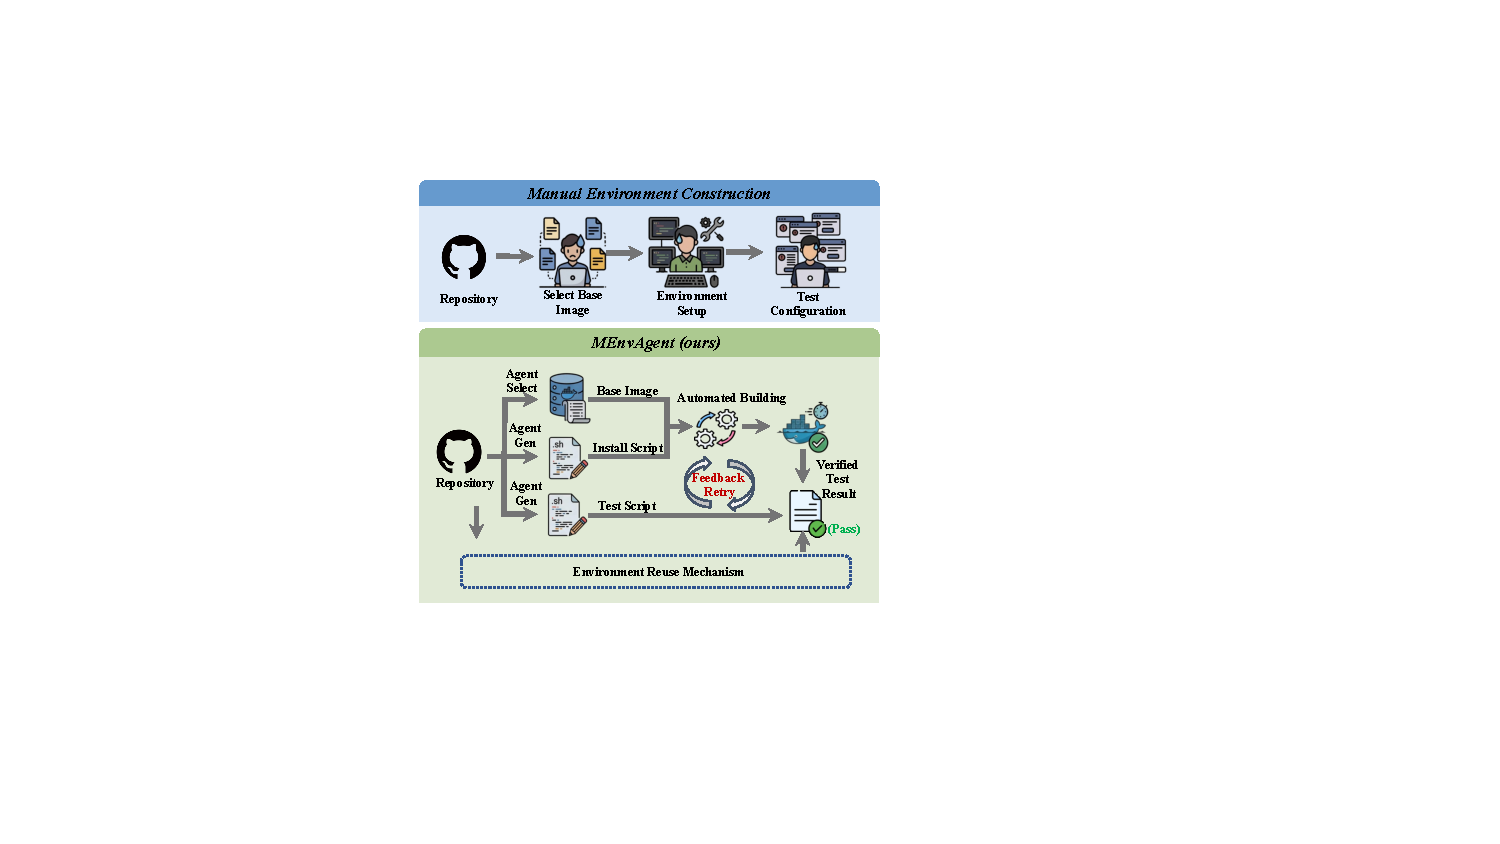
\includegraphics[width=\columnwidth]{pic/MEnvAgent-intro.pdf}
  
  \caption{Comparison between manual environment construction and MEnvAgent (Ours). MEnvAgent leverages multi-agent collaboration to achieve automated environment construction, characterized by an efficient \textbf{environment reuse mechanism}.}
  \vspace*{-0.25cm}  
  \label{fig:intro}
  \vspace*{-0.25cm}  
\end{figure}
% [P2: The Necessity of Execution Environments]
Recent research highlights the potential of Reinforcement Learning with Verifiable Rewards (RLVR) \citep{wen_rlvr_2025} to further enhance model performance in interactive settings. The efficacy of such methods hinges on the availability and scale of execution environments that provide real-time feedback. However, the complexity and cost of environment construction severely bottleneck the scalability of training data equipped with execution feedback.

% [P3: Limitations of Existing Approaches]
Consequently, existing efforts to expand training data are trapped in a dilemma between verification fidelity and scalability. To bypass the high cost of environment building, some approaches resort to sub-optimal proxies such as static analysis \citep{xie_swe-fixer_2025, wei_swe-rl_2025}, yet these methods fail to capture runtime behaviors and complex logic errors. Conversely, initiatives like SWE-gym \citep{pan_training_2025} and the manually curated environments in SWE-bench prioritize high-fidelity feedback through rigid configuration. However, this labor-intensive process is inherently unscalable and predominantly restricted to the Python ecosystem, leaving a critical gap for automated, verifiable support across diverse languages.

% [P4: The Fundamental Hurdles]
Automated Polyglot Environment Construction is thus imperative but remains challenging due to two hurdles:
(1) Knowledge-Intensive Complexity. Navigating diverse dependency systems across heterogeneous repositories requires deep expertise. The non-standardized nature of open-source projects frequently leads to intricate build failures (e.g., version conflicts) and diverse testing protocols, where invoking and validating tests differs significantly across frameworks. This complexity results in consistently low success rates, particularly in polyglot scenarios.
(2) Time-Intensive Overhead. The build process is inherently prolonged by compilation and installation steps. Furthermore, environments are fragile; a single error often necessitates a costly "clean-slate" restart, creating a prohibitive bottleneck for large-scale data expansion.

% [P5: MEnvAgent Introduction]
In this paper, we introduce \textbf{MEnvAgent}(see details in \S \ref{sec:menvagent}), an automated framework designed to achieve scalable, polyglot environment construction. MEnvAgent operates on a multi-agent architecture featuring an organic \textit{Planning-Execution-Verification} closed loop. Within this loop, specialized agents fulfill distinct responsibilities to iteratively diagnose and autonomously resolve build errors, empowering the scaling of verifiable SWE data to advance broader software engineering tasks.

% [P6: The Reuse Mechanism - Core Innovation]
Crucially, we diverge from existing approaches that construct environments for every instance from scratch. Recognizing the high degree of environmental similarity shared among related data, we propose a novel \textbf{Environment Reuse Mechanism}(see details in \S \ref{subsec:EnvReuse}). By retrieving similar historical environments and performing incremental adaptation, this mechanism effectively bridges the gap between the retrieved base and the target requirements. This paradigm shift avoids the prohibitive costs and unpredictable errors associated with scratch building, thereby simultaneously boosting success rates and efficiency.

% [P7: Benchmark & Evaluation]
To rigorously evaluate our approach and advance the field, we construct \textbf{MEnvBench}(see details in \S \ref{sec:menvbench}), a comprehensive benchmark comprising 1,000 tasks across 10 mainstream languages. Through multi-dimensional sampling, we ensure MEnvBench achieves high coverage and diversity. Extensive evaluations demonstrate that MEnvAgent outperforms state-of-the-art baselines across all languages, improving Fail-to-Pass (F2P) rates by \textbf{8.6\%} while reducing time costs by\textbf{ 43\%}. Furthermore, we leverage MEnvAgent to construct a training dataset and fine-tune open-source models, observing significant performance gains on downstream SWE tasks.

% [P8: Contributions]
The main contributions of this paper are summarized as follows:
\begin{itemize}[leftmargin=13pt, topsep=0pt, itemsep=0pt, parsep=3pt] 
    \item We introduce \textbf{MEnvAgent}, a multi-agent environment construction framework covering 10 programming languages, based on a \textit{Planning-Execution-Verification} architecture. Notably, it introduces an adaptive environment reuse mechanism for the first time.
    \item We present \textbf{MEnvBench}, the first comprehensive benchmark for evaluating multi-language environment building and test execution. This dataset covers 10 mainstream languages across 200 open-source repositories, comprising a total of 1,000 tasks.
    \item We release \textbf{MEnvData-SWE}, a high-quality, polyglot SWE dataset equipped with verified executable environments and agent trajectories to facilitate research in software engineering agents.
\end{itemize}

% \section{Problem Formulation}
% % define the task of environment construction
% In this section, we define the task of environment construction. Extending the definition from Repo2Run\cite{hu_repo2run_2025}, given a target repository $R$, the objective is to determine a suitable \textbf{base image $B$}, a \textbf{building process $P$}, and a \textbf{test configuration $T$}.
% % equation
% We formalize this goal as finding the triplet $(B, P, T)$ that satisfies:
% \begin{equation}
%     \varepsilon(R, S, T) = 0, \quad \text{where } S = \delta(B, P)
%     \label{eq:env_test_formulation}
% \end{equation}

% Here, $\delta$ is the state transition function, and the condition $\varepsilon(R, S, T) = 0$ indicates that the built environment $S$ is successfully verified by passing the specific tests defined in $T$.
% % define valid(f2p) meric for swe data
\section{Problem Formulation}
% define the task of environment construction
In this section, we define the task of environment construction. 
We extend the definition from Repo2Run\cite{hu_repo2run_2025} to better align with real-world scenarios. 
Unlike Repo2Run, which applies a fixed test configuration across all repositories, we integrate the synthesis of the test configuration $T$ into the task definition.
Consequently, given a target repository $R$, the objective is to jointly determine a suitable \textbf{base image $B$}, a \textbf{building process $\mathcal{P}$}, and a specific \textbf{test configuration $T$}.
% equation
We formalize this goal as finding the triplet $(B, \mathcal{P}, T)$ that satisfies:
\begin{equation}
    \varepsilon(R, S, T) = 0, \quad \text{where } S = \delta(B, \mathcal{P})
    \label{eq:env_test_formulation}
\end{equation}
Here, $\delta$ is the state transition function, and the condition $\varepsilon(R, S, T) = 0$ indicates that the built environment $S$ is successfully verified by passing the specific tests defined in $T$.

% \section{MEnvAgent }
\section{MEnvAgent Design}
\label{sec:menvagent}
In this section, we introduce the design of MEnvAgent. Given a code repository, MEnvAgent builds an executable environment image by generating and successfully executing a runnable environment installation script, guided by real-time environment feedback, and subsequently synthesizes a corresponding test configuration script.

\subsection{Multi-Agent Architecture}
The architecture of MEnvAgent is structured into three iterative stages: Planning, Execution, and Verification.
\begin{figure*}[t]
  \centering
  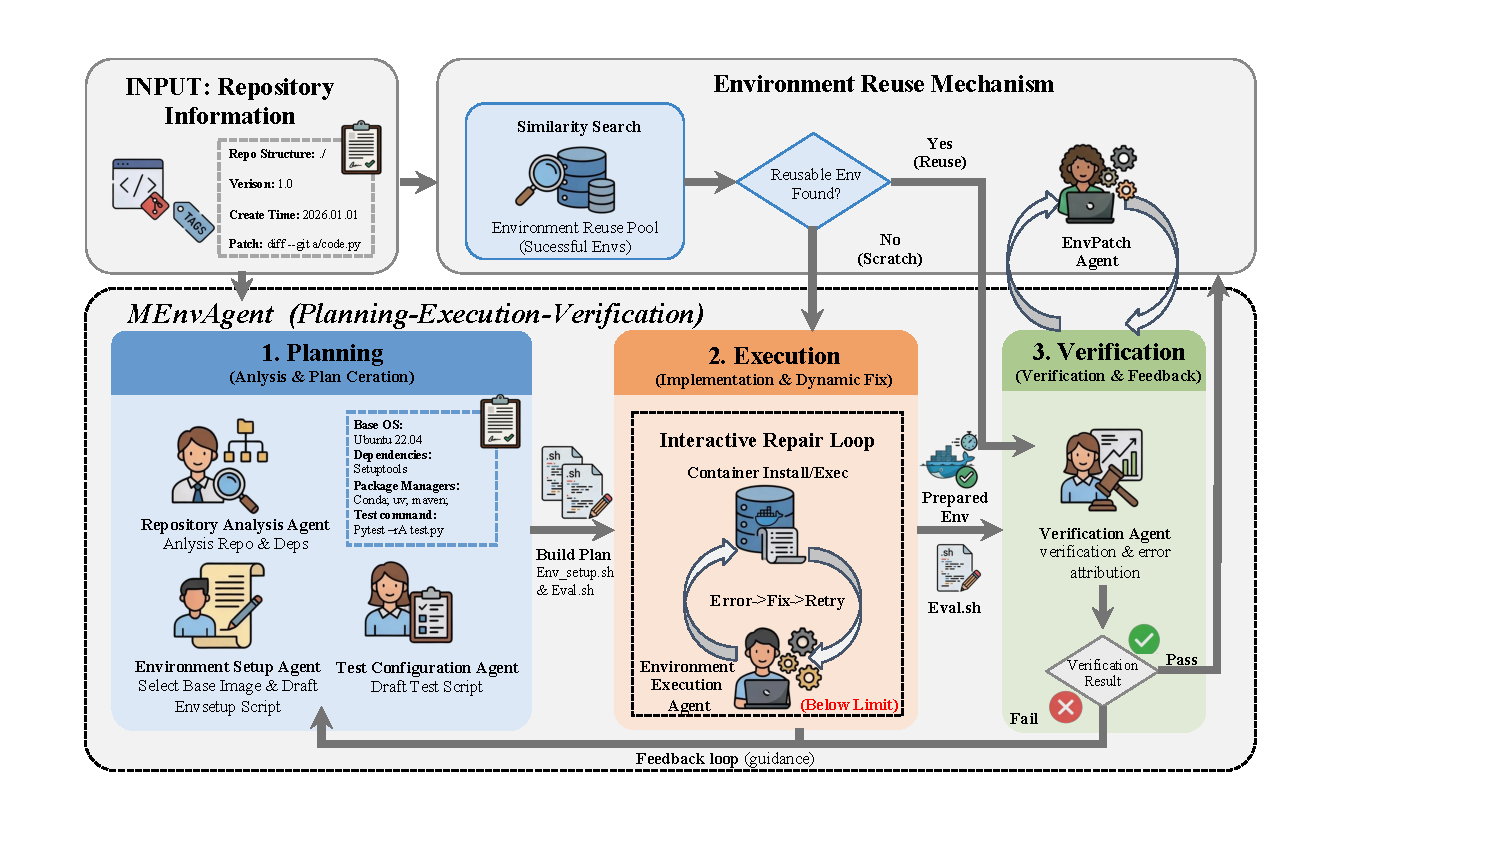
\includegraphics[width=0.95\textwidth]{pic/MEnvAgent-main.pdf}
 \caption{Overview of MEnvAgent. (Top) The Environment Reuse Mechanism retrieves and adapts historical environments via incremental patching to reduce overhead. (Bottom) The Planning-Execution-Verification loop, where agents autonomously draft scripts, interactively repair build errors, and diagnose test failures to guide iterative refinement.}
  \label{fig:menvagent_architecture}
  \vspace*{-0.25cm} 
\end{figure*}
\paragraph{Planning Stage.}
This stage is orchestrated by three specialized agents to formulate the blueprint for the environment. 
First, the \textbf{Repository Analysis Agent} explores the file structure and contents of the target repository, producing a comprehensive summary of its project type, dependency requirements, and entry points. 
This summary is passed to the downstream agents. 
Next, the \textbf{Environment Setup Agent} determines the most suitable base image and generates a complete environment installation script (denoted as $P$), which includes all necessary installation commands. 
Simultaneously, the \textbf{Test Configuration Agent} analyzes the repository structure alongside the proposed installation script to synthesize a compatible test configuration script (denoted as $T$), ensuring that the verification logic aligns with the environment setup.

\paragraph{Execution Stage.}
Once the plan is established, the system transitions to execution. 
The \textbf{Environment Execution Agent} instantiates a container based on the selected image and executes the commands in $P$. 
Crucially, this agent monitors the terminal output in real-time, capable of dynamically adjusting commands to resolve immediate execution errors (e.g., missing packages or version conflicts). 
If the installation completes successfully, the workflow proceeds to the Validation Stage. 
However, if the agent fails to resolve installation errors after multiple attempts, the process aborts the current attempt and reverts to the \textbf{Planning Stage} to regenerate a new build strategy.

\paragraph{Verification Stage.}
The final stage verifies the correctness of the built environment $S_{env}$ and the test configuration $T$. 
The \textbf{Verification Agent} executes the tests defined in $T$ within the container. 
If the tests pass (satisfying $\varepsilon(R, S_{env}, T) = 0$), the task is considered successful. 
If validation fails, the agent performs \textit{error attribution} to diagnose whether the failure stems from a missing environment dependency or an incorrect test command. 
This diagnostic feedback, along with the specific error logs, is propagated back to the \textbf{Planning Stage} to guide the agents in the next iteration. This multi-round refinement loop continues until a valid environment is successfully constructed.

% % \begin{figure*}[t] % 注意：去掉星号，变为单栏浮动体
% %     \centering
    
% %     % 第一张子图（原 Domain Diversity）
% %     \begin{subfigure}[b]{0.95\linewidth} % 宽度设为接近栏宽
% %         \centering
% %         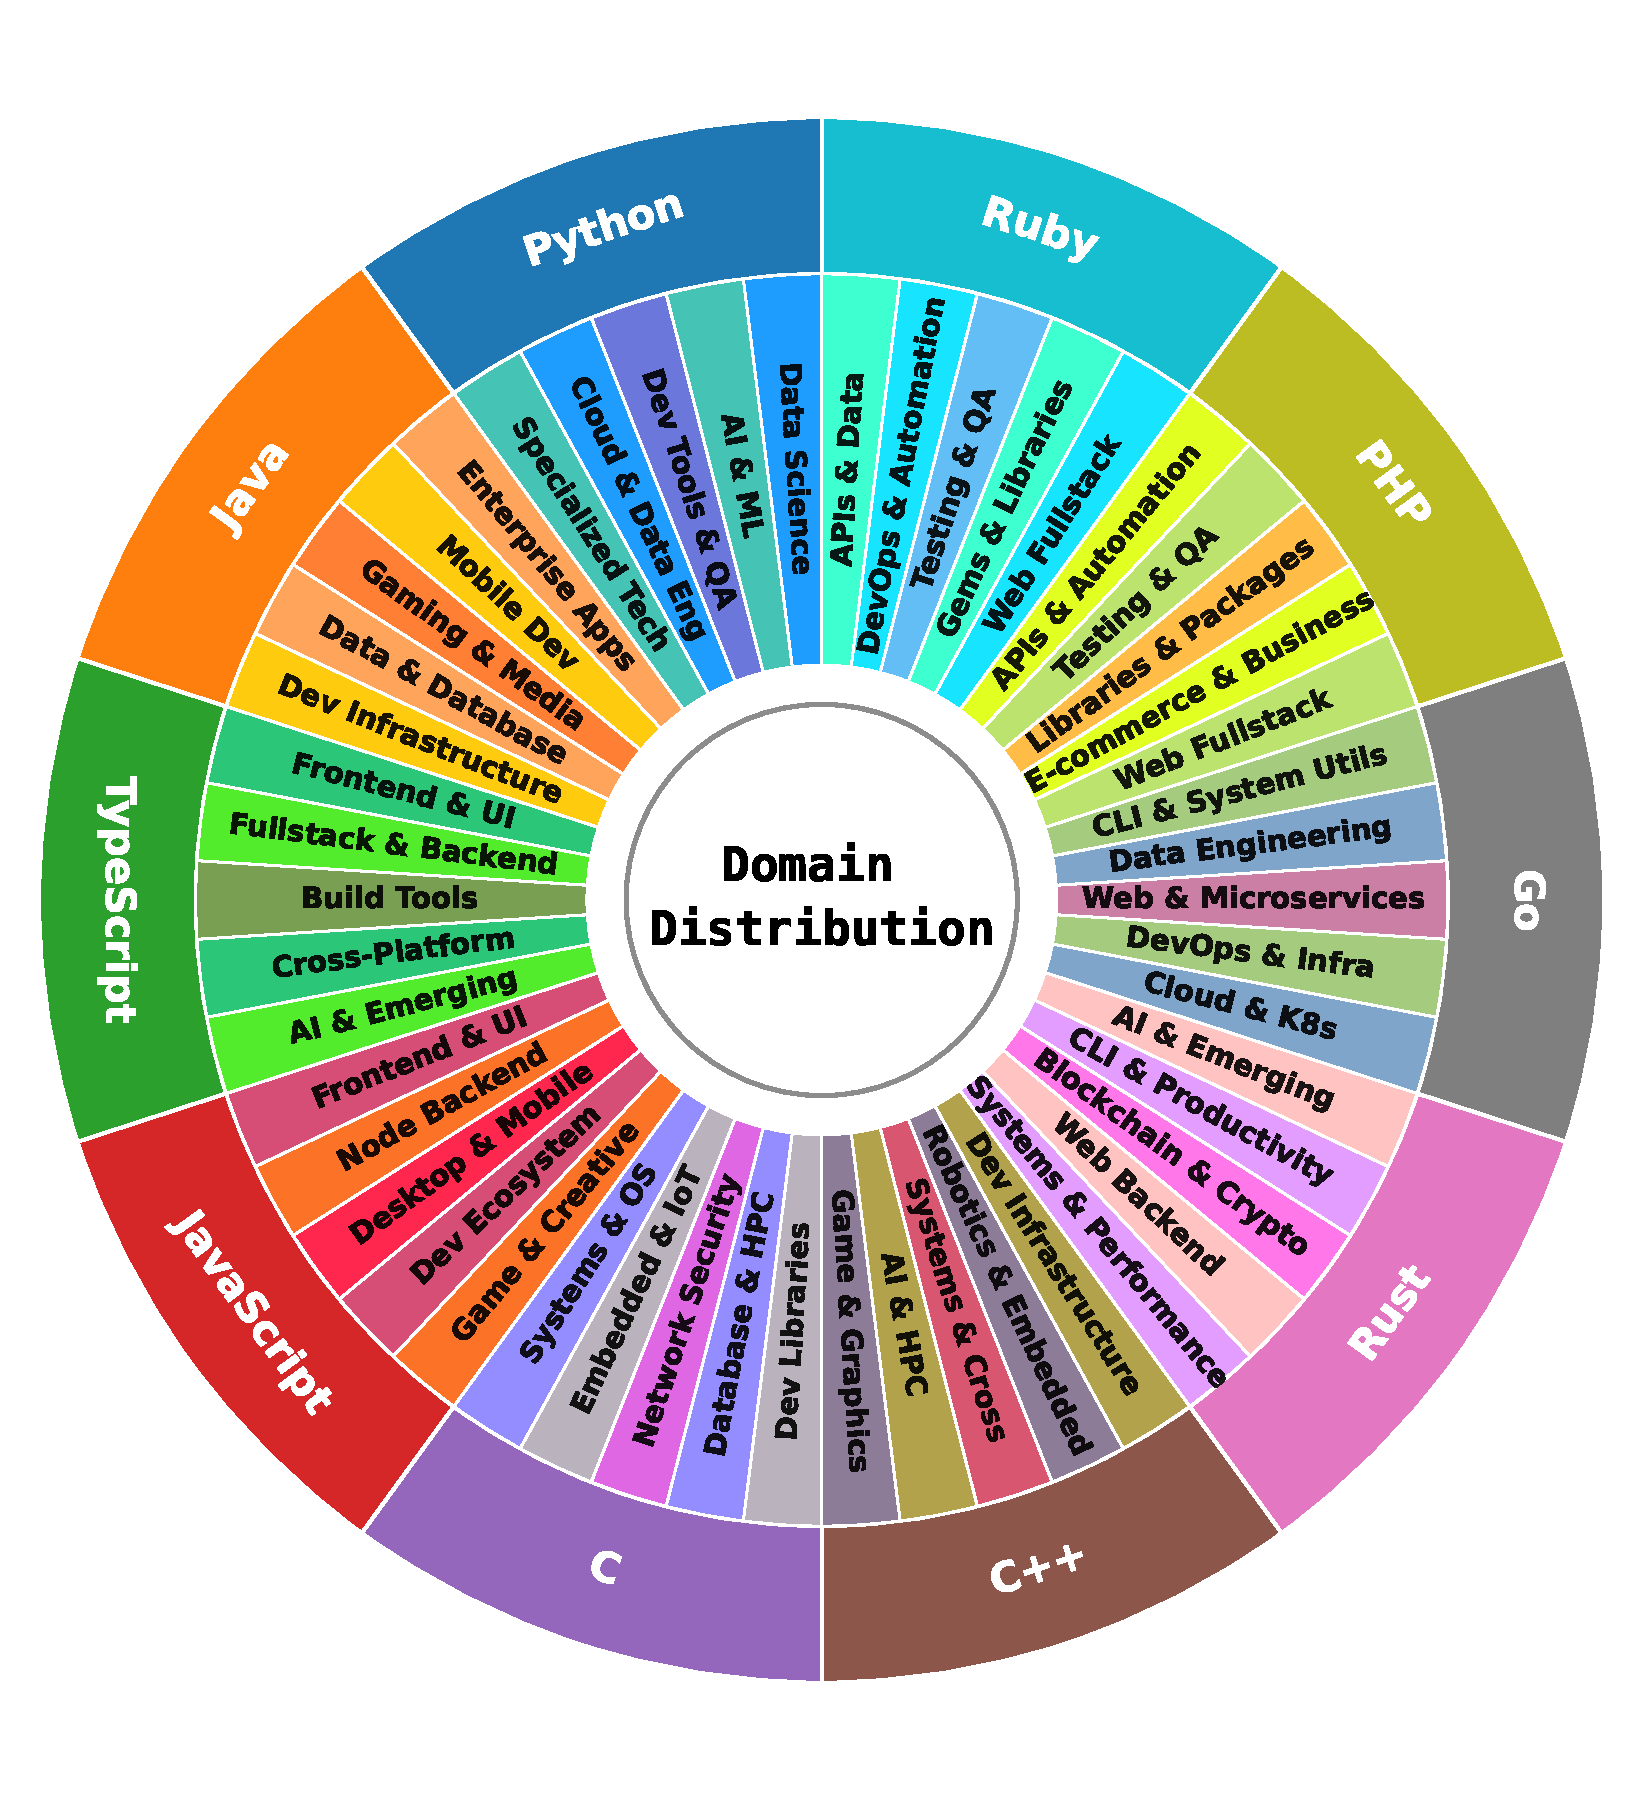
\includegraphics[width=\linewidth]{pic/domain_stats.pdf}
% %         \caption{Domain Diversity}
% %         \label{fig:stat_category}
% %     \end{subfigure}
    
% %     \vspace{0.3cm} % 添加垂直间距，防止两图太挤
% %     \par\bigskip % 强制换行
    
% %     % 第二张子图（原 Popularity Distribution）
% %     \begin{subfigure}[b]{0.95\linewidth}
% %         \centering
% %         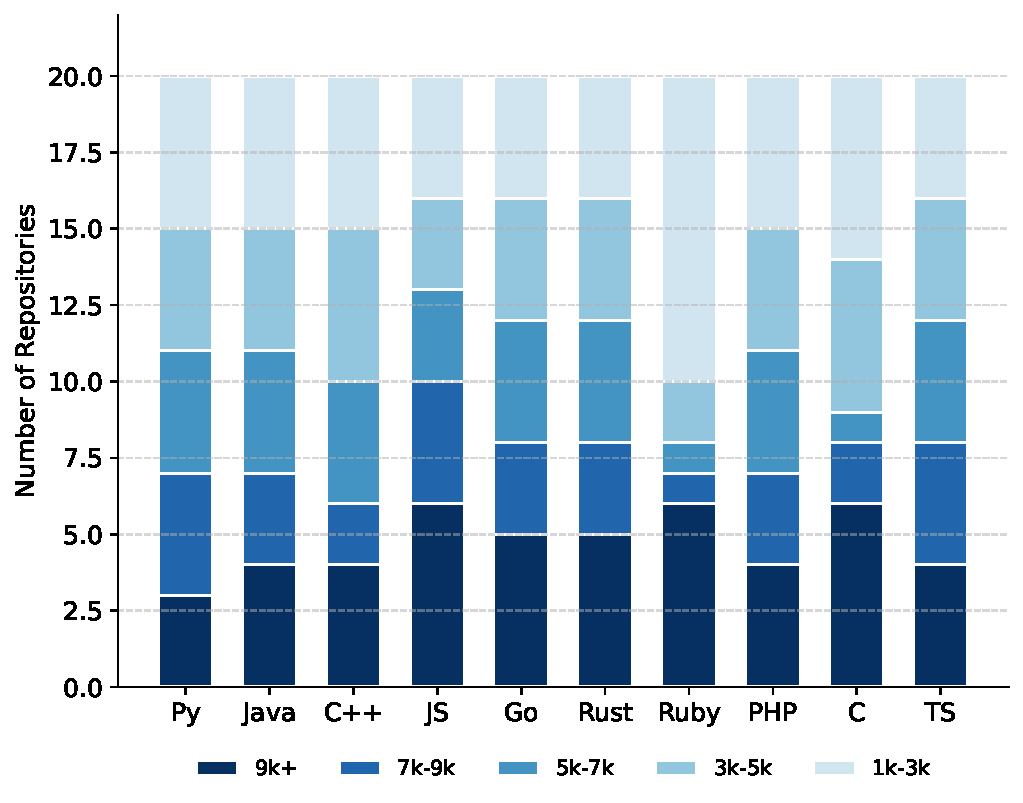
\includegraphics[width=\linewidth]{pic/popularity_stats.pdf}
% %         \caption{Popularity Distribution}
% %         \label{fig:stat_popularity}
% %     \end{subfigure}
    
% %     \caption{Distribution of MEnvBench repositories. (a) Domain Diversity ensures coverage across diverse ecosystems. (b) Popularity (Stars) validates community relevance.}
% %     \label{fig:benchmark_distribution}
% %     \vspace*{-0.3cm} 
% % \end{figure*}
% introduce Environment Reuse
% \subsection{Environment Reuse Mechanism}
% \label{subsec:EnvReuse}
% To improve success rates and efficiency, we introduce an \textbf{Environment Reuse Mechanism}. Instead of building from scratch, we identify a similar existing environment state $S_{sim}$ from environment pool.
% % EnvPatchAgent
% We employ an \textbf{EnvPatchAgent} to bridge the gap between the retrieved environment and the target repository $R$. The agent generates an incremental command sequence, denoted as the environment patch $\Delta P$. The environment building process is thus reformulated as a state transition from $S_{sim}$ to a target state $S_{new}$.
% \begin{equation}
%     S_{new} = \delta(S_{sim}, \Delta P),
%     \label{eq:env_reuse}
% \end{equation}
% where $\Delta P = \operatorname{EnvPatchAgent}(R, S_{sim})$.

% %另一个表现形式，放在文中
% % Here, $\Delta P = \operatorname{EnvPatchAgent}(R, S_{sim})$ represents the generated patch.

% The generation of $\Delta P$ follows a validation-driven process utilizing existing agents. 
% First, the Test Configuration Agent generates the test script $T$. 
% The Verification Agent then executes $T$ within the retrieved environment $S_{sim}$. 
% If the execution succeeds, $S_{sim}$ is reused directly (implying $\Delta P = \emptyset$). 
% Otherwise, the EnvPatchAgent analyzes the diagnostic feedback provided by the Verification Agent to synthesize the necessary repair commands as $\Delta P$.

% The objective is to select an $S_{sim}$ such that the resulting environment satisfies the verification condition $\varepsilon(R, S_{new}, T) = 0$, while minimizing the complexity of the patch $\Delta P$. This implies that $S_{sim}$ should maximize the semantic similarity to the required environment of $R$, allowing for successful migration with minimal modifications.

% To facilitate the reuse mechanism, we maintain an Environment Pool ($\mathcal{S}_{pool}$) of verified environments. We employ a greedy strategy grounded in software evolution patterns to identify $S_{sim}$.
% Based on Version Consistency, we first restrict the candidate set to environments from the target repository, prioritizing exact version matches. 
% Subsequently, based on Backward Compatibility, we refine the selection by identifying the environment that is strictly newer than the target base commit yet temporally closest. This strategy ensures the selected environment is compatible while minimizing divergence.

\subsection{Environment Reuse Mechanism}
\label{subsec:EnvReuse}
To avoid the high time cost and error-prone nature of deriving and executing the complete build process $\mathcal{P}$ from a raw base image $B$, we introduce an \textbf{Environment Reuse Mechanism}.
We reformulate the problem as identifying a similar existing environment state $S_{sim}$ and employing an \textbf{EnvPatchAgent} to generate an incremental command sequence $\Delta P$ that bridges the gap to the target repository $R$.
Formally, we seek a patch $\Delta P$ that transitions the retrieved environment to a valid state $S_{new}$ satisfying:
\begin{equation}
    \varepsilon(R, S_{new}, T) = 0, \quad \text{where } S_{new} = \delta(S_{sim}, \Delta P)
    \label{eq:env_test_formulation}
\end{equation}
Here, $\Delta P = \operatorname{EnvPatchAgent}(R, S_{sim})$.

Our approach executes this mechanism through two stages: Environment Retrieval and Verification-Driven Adaptation.

% % --- Part 1: Formulation (总述：只保留核心定义和流程概览) ---
% As defined in Section~\ref{sec:formulation}, the general formulation requires solving for the complete build process $\mathcal{P}$ starting from a raw base image $B$. However, this approach is often computationally expensive and error-prone.
% To address this, we introduce the \textbf{Environment Reuse} mechanism.
% Instead of constructing environments from scratch, we reformulate the problem as identifying a similar existing environment state $S_{sim}$ and employing an \textbf{EnvPatchAgent} to generate an incremental command sequence $\Delta P$ that bridges the gap between the retrieved environment and the target repository $R$.
% Formally, we seek a patch $\Delta P$ that transitions the environment to a valid state $S_{new}$ satisfying:


% --- Part 2: Retrieval (阶段一：目标 + 策略) ---
\paragraph{Environment Retrieval.}
We maintain an Environment Pool ($\mathcal{S}_{pool}$) containing previously verified environments. 
% [这里插入了你移动过来的段落，作为检索策略的动机]
The core objective of this phase is to minimize the complexity of the subsequent patch $\Delta P$. This necessitates selecting an $S_{sim}$ that maximizes dependency compatibility to the target environment, ensuring minimal modifications.
To achieve this, we employ a greedy strategy grounded in software evolution patterns.
First, prioritizing Version Consistency, we search for exact version matches associated with the target repository.
If no exact match is found, we leverage Backward Compatibility to refine the selection by identifying an environment that is strictly newer than the target base commit yet temporally closest.

% --- Part 3: Adaptation (阶段二：保持不变) ---
\paragraph{Verification-Driven Adaptation.}
Once $S_{sim}$ is retrieved, the \textbf{EnvPatchAgent} operates within a feedback loop to generate $\Delta P$.
The process commences with the Test Configuration Agent synthesizing the test script $T$, which is subsequently executed within $S_{sim}$ by the Verification Agent.
While successful execution allows for direct environment reuse, Verification failure triggers the EnvPatchAgent to analyzes the diagnostic feedback. 
Consequently, the agent synthesizes incremental commands $\Delta P$ to remediate the environment, driving an iterative refinement process until the condition $\varepsilon(R, S_{new}, T) = 0$ is met.

% \section{MEnvBench}
\section{MEnvBench Construction}
\label{sec:menvbench}
% \begin{figure}[t]
%   \centering
%   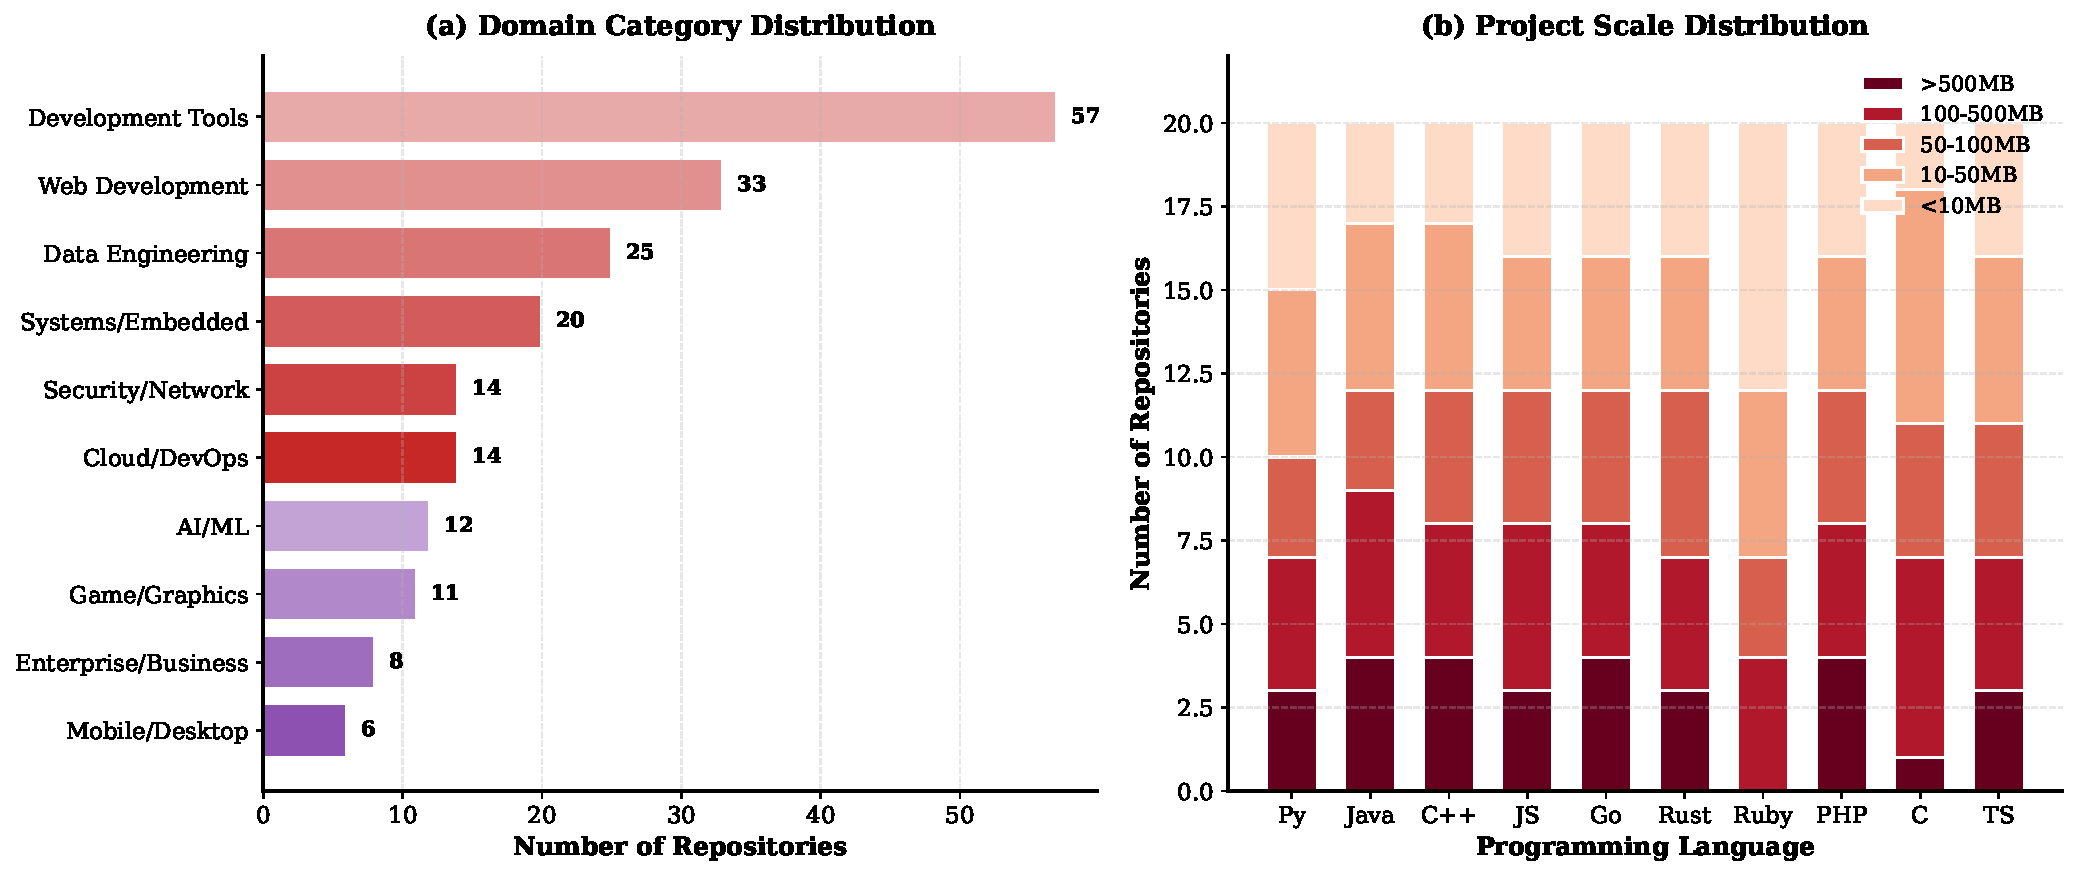
\includegraphics[width=\columnwidth]{pic/combined_distribution.pdf}
%   \caption{Comparison between manual environment construction and MEnvAgent(ours). }
%   \label{fig:intro}
%   \vspace*{-0.25cm}  
% \end{figure}

To comprehensively evaluate the capabilities of environment building agents, we present \textbf{MEnvBench}, a large-scale, polyglot benchmark designed to simulate real-world development scenarios.

\subsection{Dataset Overview}
% Overview
MEnvBench comprises \textbf{1,000} distinct environment building tasks, covering \textbf{10} mainstream programming languages. The dataset is structured hierarchically: for each language, we select \textbf{20} diverse repositories; for each repository, we extract \textbf{5} distinct instances (commits/versions). 
The allocation of 5 instances per repository represents as a strategic balance between inter-project diversity and intra-project depth. While some datasets prioritize breadth by selecting a single instance per repository (maximizing the number of unique projects), others emphasize depth by aggregating many instances from fewer repositories. Our approach seeks a middle ground: it ensures coverage of diverse repository types while simultaneously capturing sufficient intra-project variability to verify build robustness.

% \subsection{Multi-dimensional Selection Strategy}

% To ensure benchmark diversity and representativeness, we employ a Multi-dimensional Selection strategy. Instead of random selection, repositories are curated based on three dimensions: Verifiability, Scale, and Domain.

\subsection{Multi-dimensional Selection Strategy}

To ensure benchmark diversity and representativeness, we employ a Multi-dimensional Selection strategy. Instead of random selection, repositories are curated based on three dimensions: Verifiability, Domain, and Scale.

\begin{itemize}[leftmargin=13pt, topsep=0pt, itemsep=0pt, parsep=3pt] 
   \item Verifiability: We strictly mandate the presence of explicit test directories (e.g., \texttt{tests/}, \texttt{spec/}), ensuring that the constructed environment is verifiable through execution.
    
    % 在此处引用 Domain Diversity 图片
   \item Domain Diversity: We leverage LLMs to classify repositories into specific domains (e.g., Web Development, AI/ML) based on their metadata. Our sampling strategy prioritizes a wide coverage of repository types to ensure robustness across diverse software ecosystems, as shown in the distribution in Figure~\ref{fig:domain_dist}. 
    % 在此处引用 Project Scale 图片
    \item Project Scale (Size): As repository size positively correlates with build complexity, we sample across five size bands (from $<$10MB to $>$500MB) to encompass a full spectrum of difficulty levels, as shown in Figure~\ref{fig:scale_dist}.
\end{itemize}
\begin{figure}[ht]
% \vspace*{-0.25cm} 
    \centering
    % --- 第一个子图 (a) ---
    % 将 subfigure 宽度设置为略小于一半，例如 0.48\linewidth 或 0.49\linewidth
    \begin{subfigure}[b]{0.49\linewidth}
        \centering
        % 图片宽度设置为 \textwidth，填满当前子图容器
        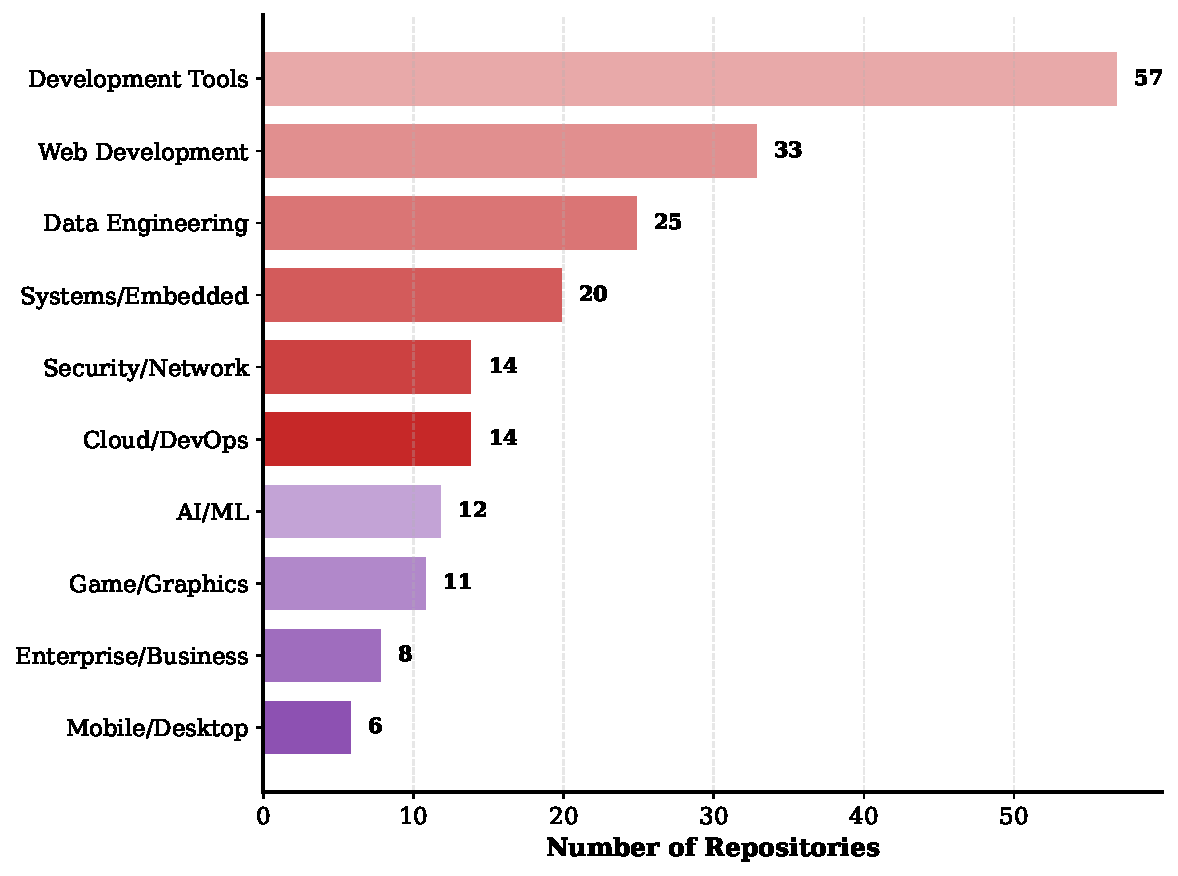
\includegraphics[width=\textwidth]{pic/category_bar_horizontal.pdf}
        \caption{Domain Diversity}
        \label{fig:domain_dist}
    \end{subfigure}
    % \hfill 用于在两个子图之间产生弹性间距，将它们推向两侧
    \hfill
    % --- 第二个子图 (b) ---
    \begin{subfigure}[b]{0.49\linewidth}
        \centering
        % 图片宽度设置为 \textwidth，填满当前子图容器
        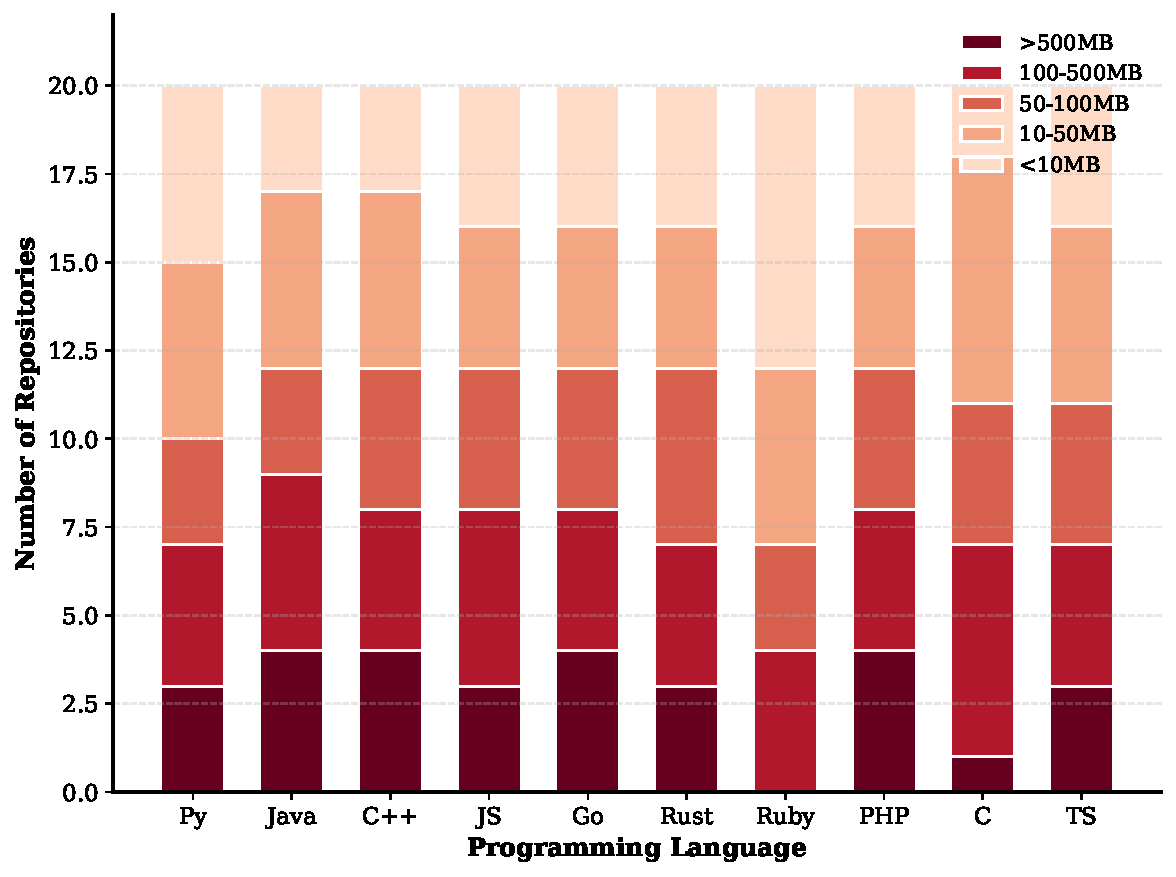
\includegraphics[width=\textwidth]{pic/scale_bar_vertical.pdf}
        
        \caption{Project Scale}
        \label{fig:scale_dist}
    \end{subfigure}
    
    % 总标题
    \caption{Overview of the dataset statistics: (a) Domain Diversity and (b) Project Scale.}
    \label{fig:comparison}
    \vspace*{-0.25cm}  
\end{figure}
% \subsection{Evaluation Metrics}
% \label{sec:metrics}

% To rigorously assess the performance of environment building agents, we employ three distinct metrics focusing on correctness, utility and efficiency. In our experimental results, these are abbreviated as \textbf{Val}, \textbf{Suc}, and \textbf{Time}, respectively.
\begin{figure*}[t]
    \centering
    % Subfigure (a): F2P Rate vs Time
    \begin{subfigure}[b]{0.48\linewidth}
        \centering
        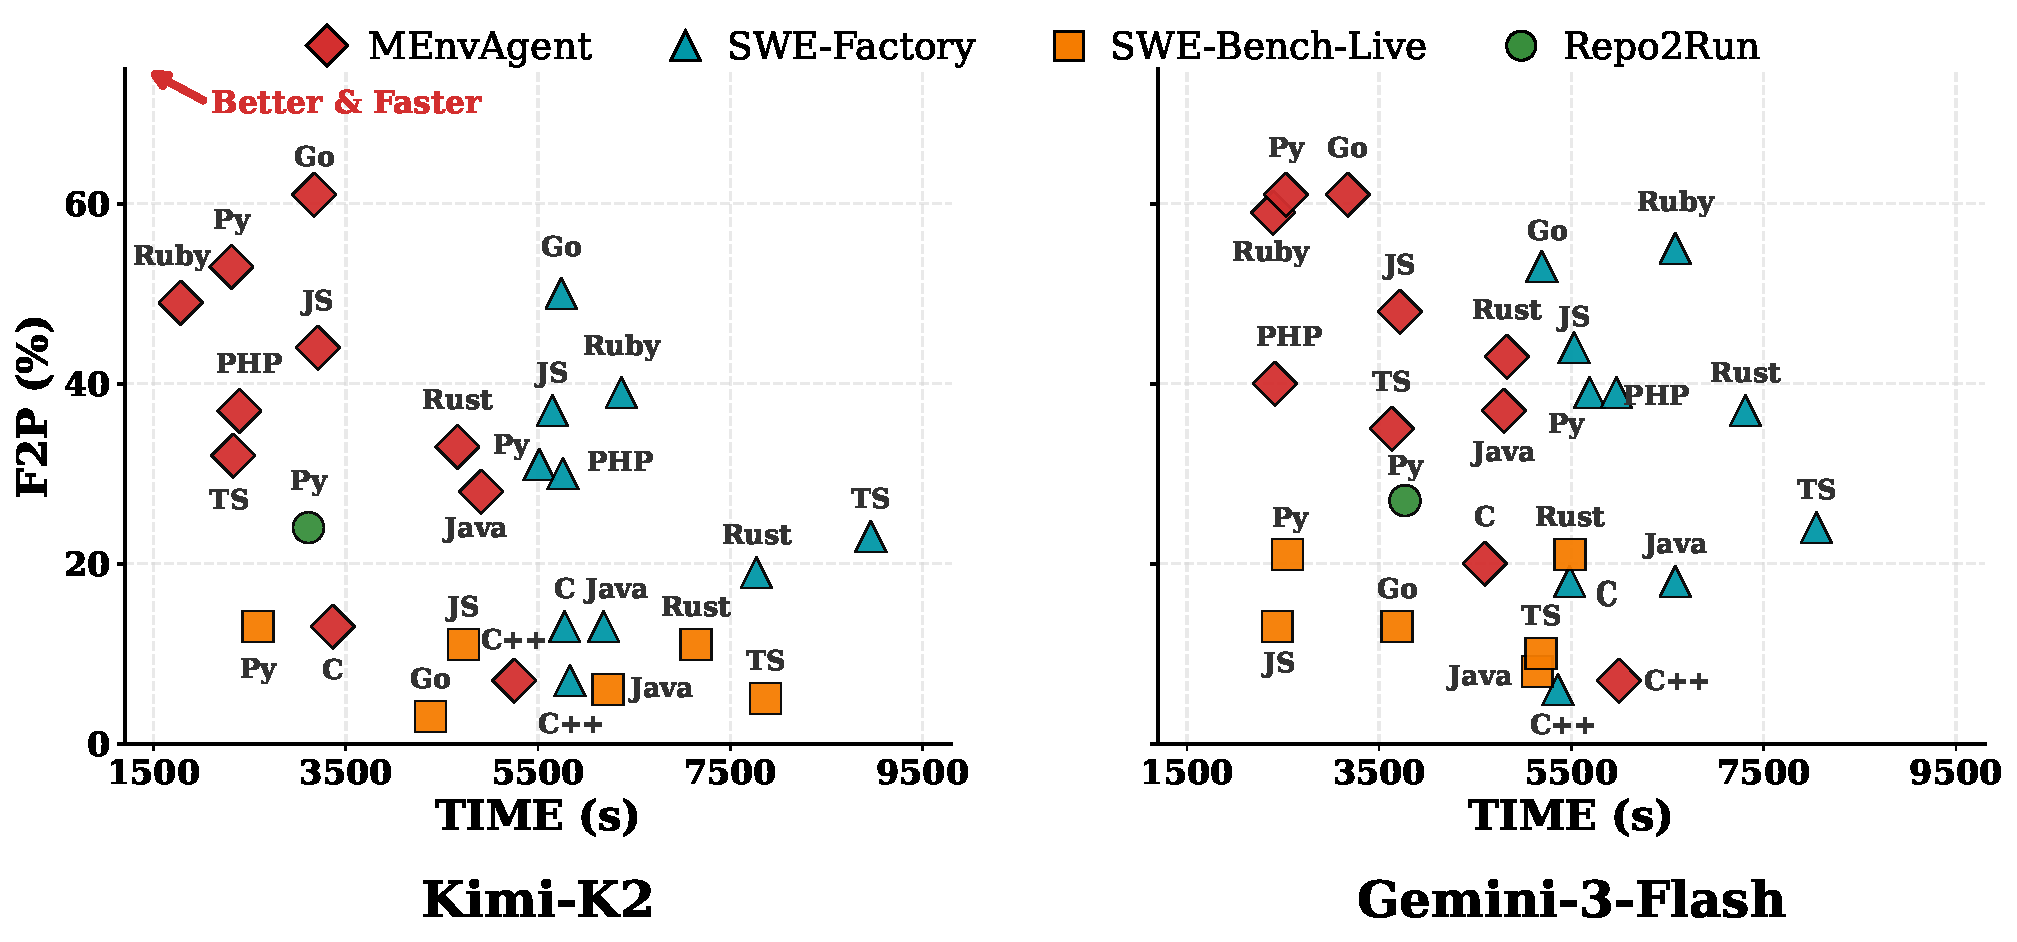
\includegraphics[width=\linewidth]{pic/chart_result_f2p_rate.pdf} 
        \caption{F2P Rate (\%) vs. Time Cost(s)}
        \label{fig:ablation_trend_a}
    \end{subfigure}
    \hfill
    % Subfigure (b): Success Rate vs Time
    \begin{subfigure}[b]{0.48\linewidth}
        \centering
        % 如果两张图用的是同一个文件占位，请记得替换为真实的第二张图
        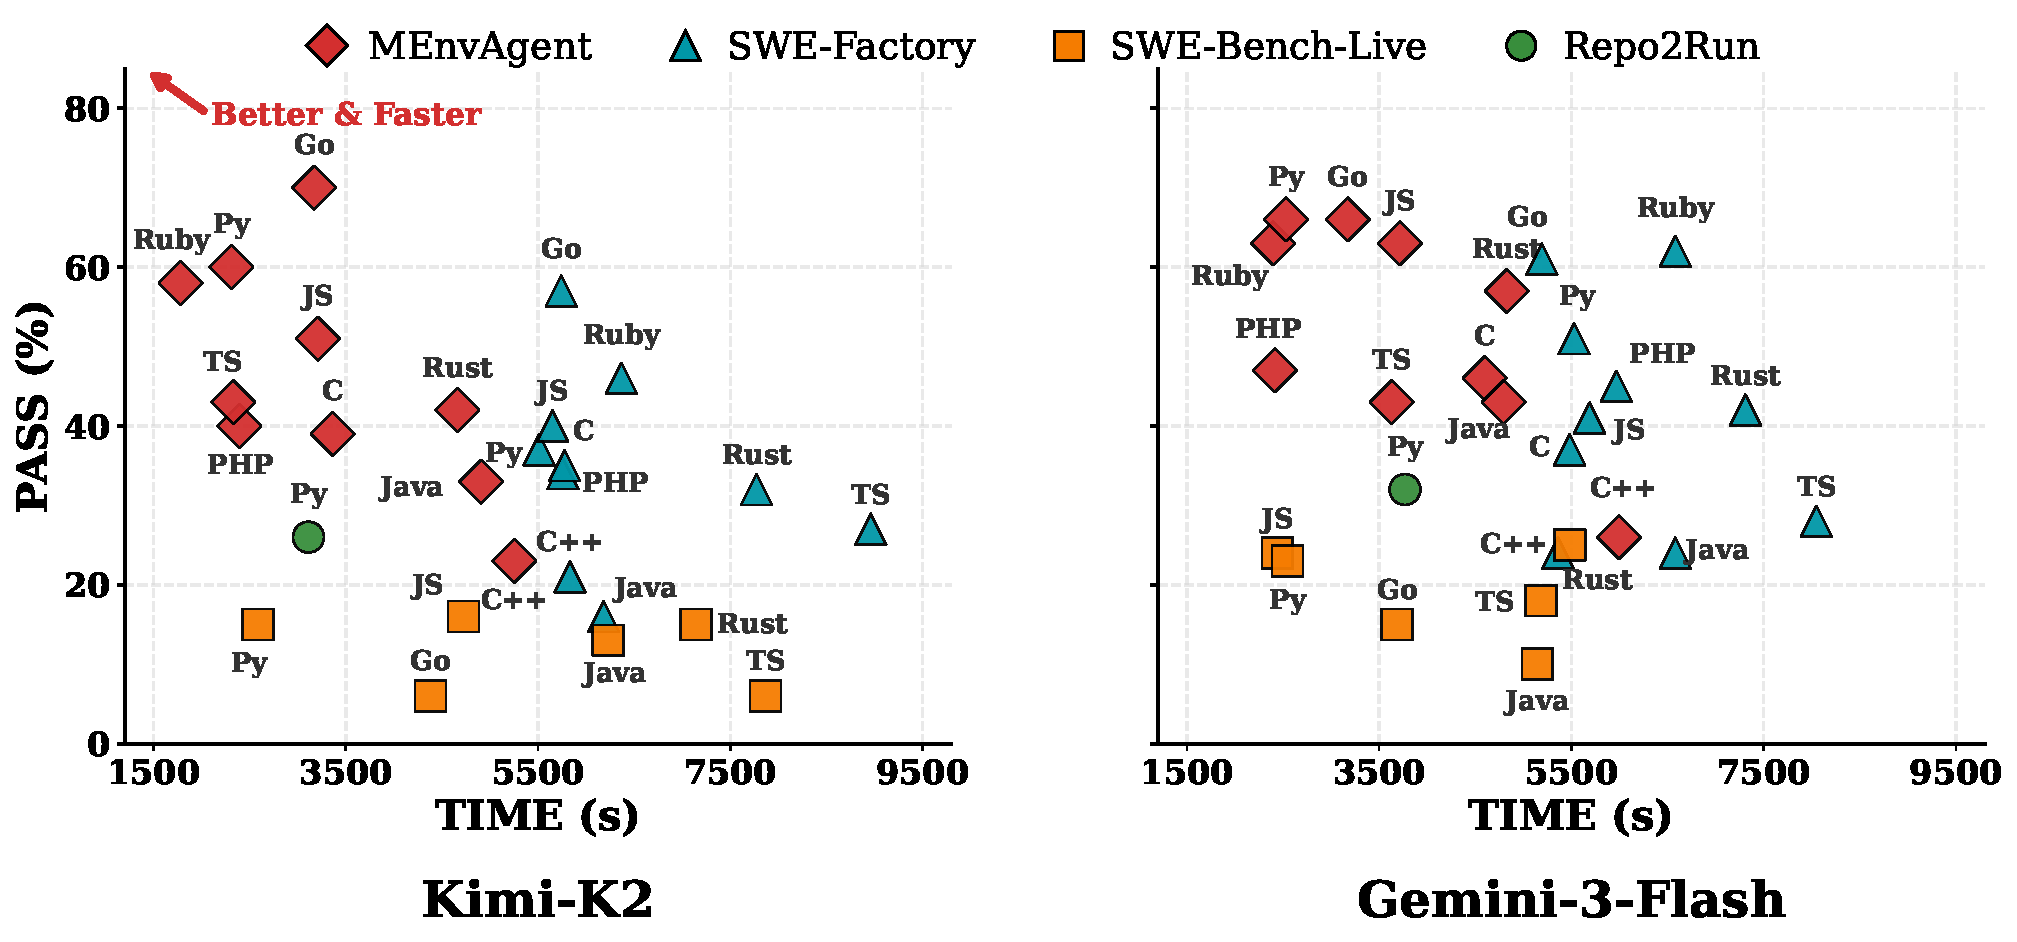
\includegraphics[width=\linewidth]{pic/chart_result_pass_rate.pdf} 
        \caption{Pass Rate (\%) vs. Time Cost(s)}
        \label{fig:ablation_trend_b}
    \end{subfigure}
    
    \caption{Performance trade-off analysis on MEnvBench. The x-axis represents the average time cost (lower is better), and the y-axis represents the pass rate (higher is better). MEnvAgent points cluster in the top-left region, indicating it achieves higher validity and success rates with significantly lower time consumption compared to baselines.}
    \label{fig:ablation_combined}
    \vspace*{-0.25cm} 
\end{figure*}
\subsection{Evaluation Metrics}
\label{sec:metrics}
We employ three metrics to evaluate performance:

\begin{itemize}[leftmargin=13pt, topsep=0pt, itemsep=0pt, parsep=3pt] 
    \item \textbf{Fail-to-Pass Rate (F2P):} 
    The most rigorous metric for assessing environment validity. 
    A task achieves F2P if and only if it satisfies \textit{differential testing}: the environment must fail the tests with the test patch (reproduction) and pass them with the fix patch (verification). 
    This metric guarantees that the constructed environment serves as a reliable testbed for verifying downstream SWE tasks.

    \item \textbf{Pass Rate (PASS):} 
    Quantifies the baseline runnability. 
    It is defined as the percentage of tasks where the constructed environment successfully passes tests with the fix patch. 
    Unlike F2P, this metric ignores the reproduction of the failure state, focusing exclusively on the final execution success rather than the complete differential verification.

    \item \textbf{Time Cost (TIME):} 
    The average wall-clock time consumed per task, serving as an indicator of the framework's operational efficiency.
\end{itemize}

\section{Experiment}
We design our experiments to answer two key research questions: 
% (1) \textbf{Effectiveness:} How does MEnvAgent compare to state-of-the-art baselines in constructing environments across diverse programming languages on MEnvBench? 
% (2) \textbf{Utility:} Can MEnvAgent facilitate the generation of high-quality training data at scale to improve the SWE capabilities of LLM?
(1) How does MEnvAgent compare to state-of-the-art baselines in constructing environments across diverse programming languages on MEnvBench? 
(2) Can MEnvAgent facilitate the generation of high-quality training data to improve the SWE capabilities of LLM?
\subsection{Evaluation on MEnvBench}
\paragraph{Model Details.}
To assess the robustness and generalization of our framework, we employ two representative Large Language Models (LLMs) as the reasoning backbone for the agents. 
For the open-source model, we select Kimi-K2, which demonstrates superior capability in agentic planning and long-context understanding. 
For the closed-source model, we utilize Gemini-3-Flash. We selected this model because it represents the latest state-of-the-art capabilities while maintaining low latency and high cost-efficiency, which are critical prerequisites for scalable environment construction scenarios.
\paragraph{Baseline Methods.}
We compare MEnvAgent against three categories of baselines: 
(1) \textbf{Repo2Run}\cite{hu_repo2run_2025}, a Python-specialized tool evaluated exclusively on the Python subset due to its extensibility constraints; 
(2) \textbf{SWE-Bench-Live}\cite{zhang_swe-bench_2025}, which supports 6 of the languages in MEnvBench, allowing for a multi-language sub-evaluation; 
and (3) \textbf{SWE-Factory}\cite{guo_swe-factory_2025}, a state-of-the-art agent framework. Although SWE-Factory natively supports only 4 languages, we extended it to support all 10 languages in MEnvBench to ensure a comprehensive and rigorous comparison. For detailed hyperparameter settings and experimental configurations, please refer to Appendix~\ref{append:experiment_setup}.
\begin{table}[t]
    \centering
    \caption{Averaged performance comparison across 10 languages. The values in parentheses indicate the improvement over the SWE-Factory baseline. 
    % \textbf{Note:} For \textit{F2P} and \textit{Pass}, we report the \textbf{absolute increase} in percentage points ($\Delta$); for \textit{Time}, we report the \textbf{relative reduction} in cost (\%).
    }
    \label{tab:performance_improvement_mixed}
    \resizebox{\linewidth}{!}{%
    \begin{tabular}{lccc}
        \toprule
        \multirow{2}{*}{\textbf{Method}} & \multicolumn{3}{c}{\textbf{MEnvBench}} \\
        \cmidrule(l){2-4}
        & \textbf{F2P (\%)} & \textbf{PASS (\%)} & \textbf{TIME (s)} \\
        \midrule
        % ---------------- Kimi-K2 ----------------
        \rowcolor{gray!15} \multicolumn{4}{c}{\textit{Kimi-K2}} \\
        SWE-Factory & 26.2 & 34.5 & 6356 \\
        \rowcolor{blue!5} \textbf{MEnvAgent} & \textbf{35.7} \small{(+9.5$\Delta$)} & \textbf{45.9} \small{(+11.4$\Delta$)} & \textbf{3339} \small{(-47.5\%)} \\
        \midrule
        % ---------------- Gemini-3-Flash ----------------
        \rowcolor{gray!15} \multicolumn{4}{c}{\textit{Gemini-3-Flash}} \\
        SWE-Factory & 33.3 & 41.5 & 6175 \\
        \rowcolor{blue!5} \textbf{MEnvAgent} & \textbf{41.1} \small{(+7.8$\Delta$)} & \textbf{52.0} \small{(+10.5$\Delta$)} & \textbf{3808} \small{(-38.3\%)} \\
        \midrule
        % ---------------- Average ----------------
        \rowcolor{gray!15} \multicolumn{4}{c}{\textit{Average}} \\
        SWE-Factory & 29.8 & 38.0 & 6266 \\
        \rowcolor{blue!5} \textbf{MEnvAgent} & \textbf{38.4} \small{(+8.6$\Delta$)} & \textbf{49.0} \small{(+11.0$\Delta$)} & \textbf{3574} \small{(-43.0\%)} \\
        \bottomrule
    \end{tabular}%
    }
\end{table}

\paragraph{Results on MEnvBench.}
We evaluate the overall effectiveness and efficiency of our framework on MEnvBench. The aggregated metrics are presented in Table~\ref{tab:performance_improvement_mixed}, and the efficiency-quality trade-off is visualized in Figure~\ref{fig:ablation_combined}. 
In the scatter plots, the x-axis represents the average time cost, while the y-axis denotes the Pass Rate or F2P Rate. As illustrated, MEnvAgent consistently occupies the upper-left quadrant across all backbone models and programming languages. 
This distribution signifies an optimal performance state—simultaneously achieving the highest validity while minimizing computational overhead. 
In contrast, the baselines exhibit distinct limitations: SWE-Factory is predominantly distributed in the right-hand region, indicating that while it achieves competitive runnability, it suffers from excessive latency due to inefficient trial-and-error loops. 
Meanwhile, Repo2Run and SWE-bench-live cluster in the lower region, where despite maintaining acceptable efficiency, their capability to generate valid environments is significantly compromised. This visual superiority is quantitatively corroborated by Table~\ref{tab:performance_improvement_mixed}, which compares our method directly against the strongest baseline, SWE-Factory. 
Averaged across models, MEnvAgent improves the strict F2P Rate by \textbf{8.6\%} and the Pass Rate by \textbf{11.0\%}, while simultaneously reducing time costs by \textbf{43.0\%}. 
For complete per-language statistics and granular comparisons, we refer readers to Table~\ref{tab:longbench_full} in Appendix~\ref{append:detailed_results}.





% \subsection{Evaluation on SWE Tasks}
% To further demonstrate the practical utility of our framework, we leveraged MEnvAgent to establish a scalable, fully automated pipeline for continuous construction of software engineering tasks equipped with executable environment from real-world GitHub repositories (see Appendix~\ref{append:data_production} for details).
% \paragraph{Train Dataset.}
% \paragraph{Model.}Baseline Model Qwen-3-Coder-A3B Qwen2.5-coder(7B,14,32B) GLM4; Expert Model Claude-sonnect-4.5

% \paragraph{Agent system.} OpenHands
\begin{table*}[t]
    \centering
    \footnotesize 
    \renewcommand{\arraystretch}{0.9} 
    
    \caption{\textbf{Main results on SWE benchmarks.} Performance is measured by Resolved Rate (\%). Params denotes Total and Active parameters (in Billions). \textbf{V} and \textbf{M} denote the Verified and Multilingual versions, respectively. Best results are \textbf{bolded}.}
    \label{tab:main_results}
    
    \vspace{-0.2cm}
    
    \resizebox{\textwidth}{!}{
    % 1. 去掉竖线：将 {l|cc|cc|cc} 改为 {l cc cc cc}
    \begin{tabular}{l rr rr rr}
    \toprule
    \multirow{2}{*}{\textbf{Model}} & \multicolumn{2}{c}{\textbf{Params (B)}} & \multicolumn{2}{c}{\textbf{SWE-Bench (V)}} & \multicolumn{2}{c}{\textbf{SWE-Bench (M)}} \\
    
    % 2. 增加 cmidrule：因为去掉了竖线，需要用横线来表示分组
    % (lr) 表示线条左右缩进，避免连在一起
    \cmidrule(lr){2-3} \cmidrule(lr){4-5} \cmidrule(lr){6-7}
    
    & \textbf{Total} & \textbf{Active} & \textbf{Base} & \textbf{SFT} & \textbf{Base} & \textbf{SFT} \\
    \midrule
    Qwen2.5-Coder-7B-Instruct\cite{5team2025glm45agenticreasoningcoding} & 7 & 7 & 0.0 & \textbf{21.8} & 0.0 & \textbf{12.3} \\
    Qwen2.5-Coder-14B-Instruct\cite{5team2025glm45agenticreasoningcoding} & 14 & 14 & 5.8 & \textbf{39.8} & 0.0 & \textbf{31.2} \\
    Qwen2.5-Coder-32B-Instruct\cite{5team2025glm45agenticreasoningcoding} & 32 & 32 & 7.5 & \textbf{54.6} & 0.0 & \textbf{38.3} \\
    Qwen3-Coder-30B-A3B-Instruct\cite{5team2025glm45agenticreasoningcoding} & 30 & 3 & 45.2 & \textbf{53.4} & 34.7 & \textbf{38.0} \\
    GLM-4.5-Air\cite{5team2025glm45agenticreasoningcoding} & 106 & 12 & 58.0  & \textbf{62.8} & 42.3 & \textbf{47.7} \\
    \bottomrule
    \end{tabular}
    }
    \vspace{-0.3cm}
\end{table*}
% \paragraph{Results.}
\subsection{Evaluation on SWE Tasks}
\label{subsec:eval_swe}
To explore the utility of MEnvAgent for training software engineering agents, we employ \textbf{rejection sampling fine-tuning} as the primary procedure for improving base LLMs, following the methodology established in prior works~\cite{yang_swe-smith_2025,guo_swe-factory_2025,wang_swe-mirror_2025}.
Our experiment workflow is as follows. 
First, we leveraged MEnvAgent to establish a fully automated pipeline for the continuous construction of verifiable software engineering tasks from real-world GitHub repositories (see Appendix~\ref{append:data_production} for details). 
Through this pipeline, we constructed \textbf{MEnvData-SWE}, a diverse dataset of task instances equipped with executable environments across 10 programming languages.
Next, we run an agent framwork with an expert model on MEnvData-SWE. 
At this step, the trajectory corresponding to each run is recorded. Then, we fine-tune
the base (or “student”) model on the approximately 3k trajectories corresponding to resolved instances and evaluated them on separate benchmarks.

\paragraph{Models.} 
For the expert model, we employ \textbf{Claude-4.5-Sonnet}~\cite{TODO_citation}, representing the state-of-the-art in coding capabilities. 
For base models, we select a diverse array of architectures to verify robustness: the dense Qwen-2.5-Coder-Instruct series (7B, 14B, and 32B), the MoE-based Qwen-3-Coder-30B-A3B-Instruct, and GLM-4.5-Air. 
Training and hyperparameter details are provided in Appendix~\ref{append:training_details}.

\paragraph{Agent Scaffolding.} 
We use \textbf{OpenHands}~\cite{wang_openhands_2024}
, an event-driven agent framework for solving software engineering tasks. 
OpenHands provides the LLM with a sandboxed operating system and a set of tools to interact with the codebase effectively. 
At each turn, the agent generates a thought and an action, where the action involves editing files (via \texttt{str-replace-editor}), executing shell commands (via \texttt{execute-bash}), or submitting the task (via \texttt{finish}). 
We chose OpenHands as it establishes strong baselines on benchmarks like SWE-Bench. 

\paragraph{Evaluation Benchmarks.} 
We evaluate our models on two primary benchmarks. 
The first, \textbf{SWE-bench Verified}~\cite{chowdhury2024swebenchverified}, is a high-quality, human-curated set of 500 real-world software engineering issues in Python, selected for their reliable evaluation properties. 
The second, \textbf{SWE-bench Multilingual}~\cite{swebench_multilingual}, is a benchmark designed to assess generalization capabilities beyond Python. It consists of task instances covering 9 additional programming languages. 
We report the \textbf{Resolved Rate (\%)}, which is the proportion of tasks where the agent's submitted patch passes all acceptance tests.
It is worth noting that we rectified a \texttt{git log} manipulation issue within the evaluation environment. Consequently, our reported scores may be slightly lower than the official baselines due to this more rigorous evaluation setting.
% \begin{table}[t]
%     \centering
%     \caption{\textbf{Evaluation results on SWE benchmarks.} We report the Resolved Rate (\%) for models of varying scales. Params T/A denotes Total and Active parameters (in Billions). The best results for each model size are bolded.}
%     \label{tab:main_results}
%     \resizebox{\linewidth}{!}{
%     \begin{tabular}{l|cc|cc|cc}
%     \toprule
%     \multirow{2}{*}{\textbf{Model}} & \multicolumn{2}{c|}{\textbf{Params (B)}} & \multicolumn{2}{c|}{\textbf{SWE-Ver.}} & \multicolumn{2}{c}{\textbf{SWE-Mul.}} \\
%     & \textbf{T} & \textbf{A} & Base & \textbf{SFT} & Base & \textbf{SFT} \\
%     \midrule
%     Qwen2.5-Coder & 7 & 7 & 25.4 & \textbf{32.1} & 18.2 & \textbf{24.5} \\
%     Qwen2.5-Coder & 14 & 14 & 30.5 & \textbf{41.2} & 22.1 & \textbf{31.8} \\
%     Qwen2.5-Coder & 32 & 32 & 35.2 & \textbf{52.4} & 28.5 & \textbf{40.6} \\
%     Qwen-3-Coder & 30 & 3 & 40.1 & \textbf{48.5} & 33.2 & \textbf{41.9} \\
%     GLM-4.5-Air & 106 & 12 & 42.5 & \textbf{50.2} & 35.8 & \textbf{43.7} \\
%     \bottomrule
%     \end{tabular}
%     }
% \end{table}

\paragraph{Results.} 
Table~\ref{tab:main_results} presents the comparative evaluation on SWE-bench Verified and Multilingual. 
Experimental results demonstrate that fine-tuning on our dataset yields significant and consistent performance gains across all model sizes and architectures.
Notably, for the Qwen-2.5-Coder series, we observe a positive correlation between model scale and performance improvement; as the model size increases (from 7B to 32B), the magnitude of the gain becomes more pronounced, suggesting that our data effectively activates the latent potential of larger models.
Furthermore, substantial improvements are achieved even on the top-tier MoE baselines (Qwen-3 and GLM-4.5-Air) that are already state-of-the-art among models of \textbf{comparable scale}, strongly validating that MEnvData-SWE provides high-quality, domain-specific supervision capable of enhancing even the strongest existing models.


% \subsection{Evaluation on SWE Tasks}
% To further demonstrate the practical utility of our framework, we leveraged MEnvAgent to establish a fully automated pipeline for continuous construction of verifiable software engineering tasks from real-world GitHub repositories (see Appendix~\ref{append:data_production} for details).

% \paragraph{MEnvData-SWE Dataset.}
% We leveraged MEnvAgent to continuously construct software engineering tasks across \textbf{10 programming languages} from real-world GitHub repositories.
% Following established practices~\cite{swe_smith, swe_mirror}, we employed a \textbf{Rejection Sampling} strategy to curate high-quality agent trajectories.
% Using \textbf{Claude-3.5-Sonnet} as the expert agent, we generated candidate solutions and filtered them based on strict verification criteria (passing both existing and newly generated tests).
% This process yielded a diverse corpus of approximately \textbf{10k successful trajectories}, denoted as \textbf{MEnv-Instruct}, covering a wide spectrum of software ecosystems.

% \paragraph{Experimental Setup.}
% We selected the \textbf{Qwen2.5-Coder} series (3B, 7B, 14B, 32B) and \textbf{GLM-4} as base models.
% We performed full-parameter Supervised Fine-Tuning (SFT) on these models using MEnvData-SWE within the \textbf{OpenHands}~\cite{openhands2024} agent framework.
% Detailed training configurations and hyperparameters are provided in Appendix~\ref{append:training_details}.

% \paragraph{Benchmarks and Results.}
% We evaluated the fine-tuned models on two challenging benchmarks:
% (1) \textbf{SWE-bench Verified}~\cite{swebench_verified}, for Python-centric issue resolution; and
% (2) \textbf{SWE-bench Multilingual}~\cite{swebench_multilingual}, to assess generalization across different languages.
% As shown in Table~\ref{tab:swe_results}, models fine-tuned on MEnv-Instruct consistently outperform their base counterparts across both benchmarks. Notably, significant improvements are observed in the multilingual setting, validating that our dataset effectively enhances the agent's capability to handle diverse software environments beyond Python.

% \begin{table}[ht]
%     \centering
%     \caption{Performance comparison on SWE-bench Verified and Multilingual. "Base" denotes off-the-shelf models, and "Ours" denotes models fine-tuned on MEnv-Instruct.}
%     \label{tab:swe_results}
%     \resizebox{1.0\linewidth}{!}{
%     \begin{tabular}{l|c|cc|cc}
%     \toprule
%     \multirow{2}{*}{\textbf{Model}} & \multirow{2}{*}{\textbf{Size}} & \multicolumn{2}{c|}{\textbf{SWE-bench Verified}} & \multicolumn{2}{c}{\textbf{SWE-bench Multilingual}} \\
%     & & Base (\%) & Ours (\%) & Base (\%) & Ours (\%) \\
%     \midrule
%     Qwen2.5-Coder & 3B & - & - & - & - \\
%     Qwen2.5-Coder & 7B & - & - & - & - \\
%     Qwen2.5-Coder & 14B & - & - & - & - \\
%     Qwen2.5-Coder & 32B & - & - & - & - \\
%     GLM-4 & 9B & - & - & - & - \\
%     \bottomrule
%     \end{tabular}
%     }
% \end{table}
% \end{itemize}
% Predefined Script
% repo2run
% swe-bench-live
% swe-factory
% \begin{table*}[t]
%     \centering
%     \caption{Comparison of training results on SWE-bench benchmarks. The \textbf{Params} column denotes Total/Active parameters. Values in parentheses indicate the absolute improvement ($\Delta$) over the baseline.}
%     \label{tab:model_comparison_horizontal}
%     \resizebox{\linewidth}{!}{%
%     \begin{tabular}{l c ccc ccc}
%         \toprule
%         \multirow{2}{*}{\textbf{Model}} & \multirow{2}{*}{\textbf{Params (T/A)}} & \multicolumn{3}{c}{\textbf{SWE-bench Verified}} & \multicolumn{3}{c}{\textbf{SWE-bench Multilingual}} \\
%         \cmidrule(lr){3-5} \cmidrule(lr){6-8}
%         & & Base & SFT & Imp. & Base & SFT & Imp. \\
%         \midrule
%         % ---------------- Qwen3 ----------------
%         Qwen3-Coder-30B-A3B-Instruct & 30B / 3B & 45.2 & \textbf{53.4} & \small{(+8.2$\Delta$)} & 31.0 & \textbf{38.3} & \small{(+7.3$\Delta$)} \\
        
%         % ---------------- GLM4.6 ----------------
%         GLM4.6 & 355B / 32B & - & - & - & - & - & - \\
%         \bottomrule
%     \end{tabular}%
%     }
% \end{table*}
\begin{figure*}[t]
    \centering
    % 第一张子图：Reuse Success Rate (R-Suc)
    \begin{subfigure}[b]{0.32\linewidth}
        \centering
        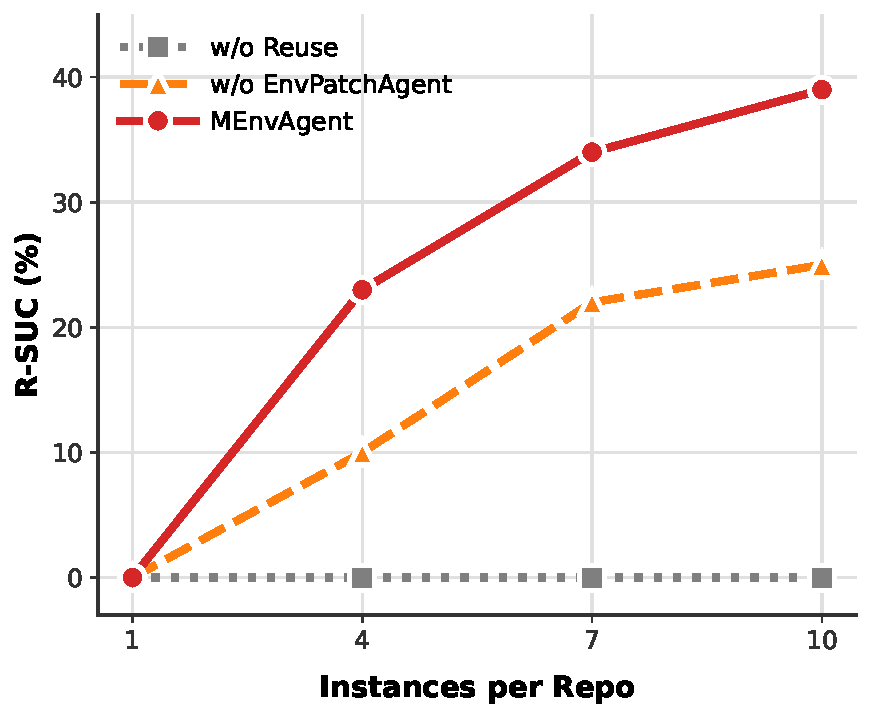
\includegraphics[width=\linewidth]{pic/ablation_reuse_success_rate.pdf}
        \caption{Reuse Success Rate}
        \label{fig:ablation_rsuc}
    \end{subfigure}
    \hfill
    % 第二张子图：Time Cost
    \begin{subfigure}[b]{0.32\linewidth}
        \centering
        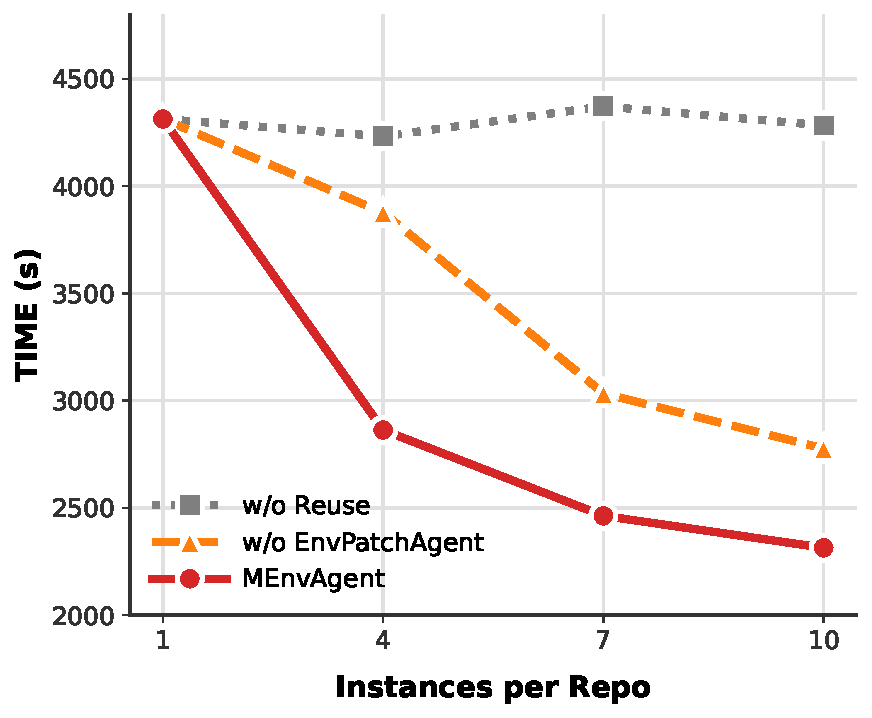
\includegraphics[width=\linewidth]{pic/ablation_time_cost.pdf}
        \caption{Time Cost}
        \label{fig:ablation_time}
    \end{subfigure}
    \hfill
    % 第三张子图：Pass Rate
    \begin{subfigure}[b]{0.32\linewidth}
        \centering
        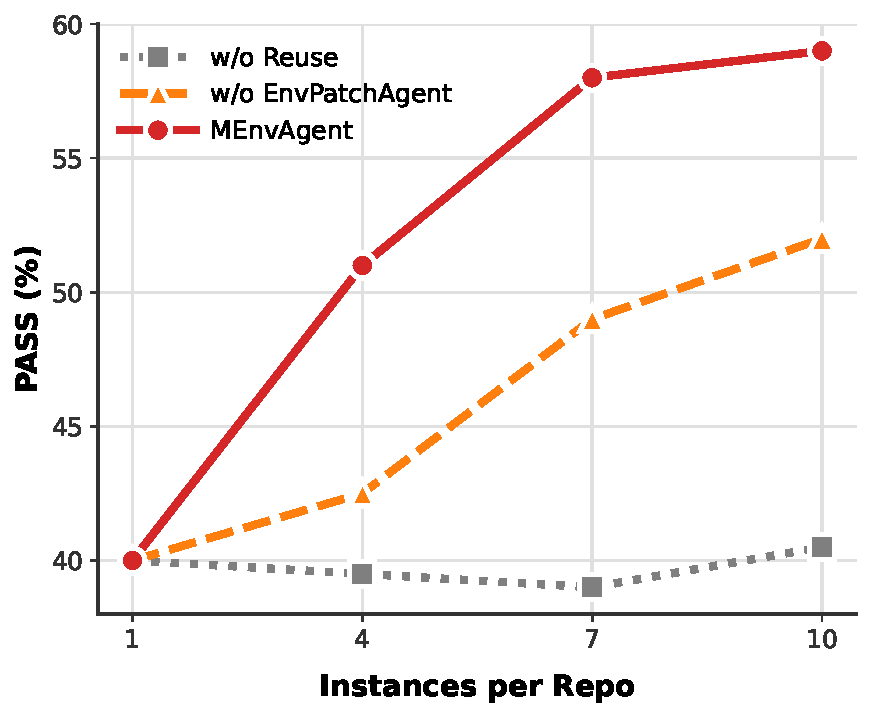
\includegraphics[width=\linewidth]{pic/ablation_pass_rate.pdf}
        \caption{Pass Rate}
        \label{fig:ablation_pass}
    \end{subfigure}
    
    \caption{Impact of data scale on performance metrics. 
    We illustrate the trends of (a) Reuse Success Rate, (b) Time Cost, and (c) Pass Rate as the number of instances per repository increases from 1 to 10. 
    The results confirm that larger data scale significantly enhance reuse probability and overall efficiency.}
    \label{fig:ablation_trend} % 对应正文中引用的 Figure \ref{fig:ablation_trend}
    \vspace*{-0.25cm} 
\end{figure*}
\section{Analysis}
\subsection{Ablation Study of Environment Reuse}
\label{sec:ablation}

To validate the effectiveness of the Environment Reuse mechanism and the critical role of the EnvPatchAgent, we conduct a comprehensive ablation study. Furthermore, we investigate how the data scale (the number of historical instances per repository) influences reuse performance.

\paragraph{Experimental Setup.}
To isolate the contribution of each component, we evaluate our framework against two ablated variants:
(1) \textbf{MEnvAgent (Full)}, our complete framework incorporating both the Environment Retrieval and the EnvPatchAgent;
(2) \textbf{w/o EnvPatchAgent (Direct)}, a variant that retrieves the most similar environment $S_{sim}$ but applies it directly without modification, validating the necessity of the patching mechanism; and
(3) \textbf{w/o Reuse (Scratch)}, the minimal baseline that disables the reuse mechanism entirely and builds every task from the base image.
To measure reuse efficacy, we employ the \textbf{Reuse Success Rate (RSR)}, defined as the proportion of tasks successfully verified via the reuse pathway without falling back to the scratch build.

% \begin{figure*}[t]
%     \centering
%     % 第一张子图：scale
%     \begin{subfigure}[b]{0.32\linewidth}
%         \centering
%         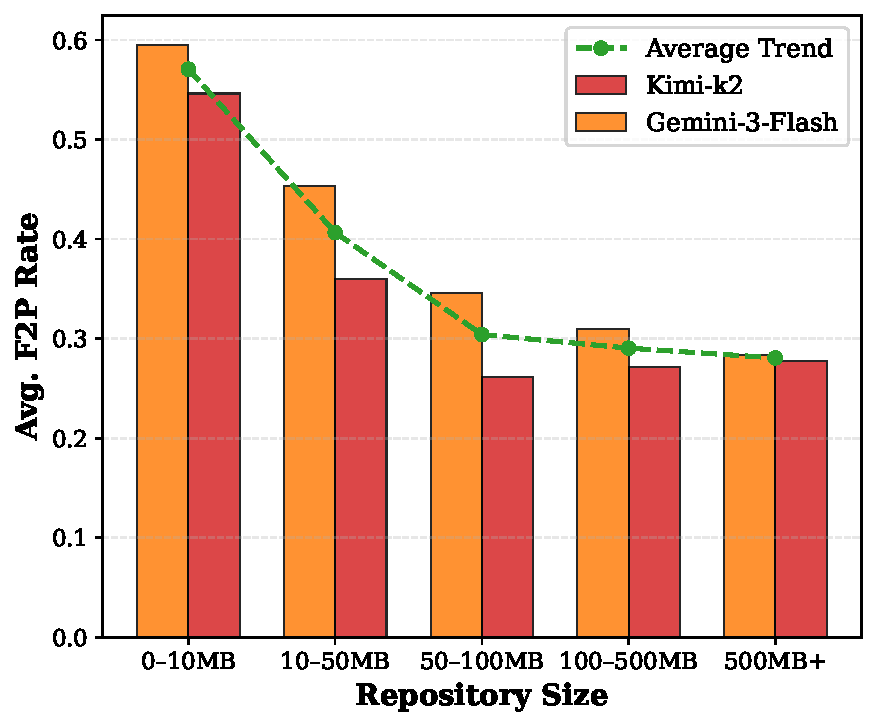
\includegraphics[width=\linewidth]{pic/repo_analysis_repo_size.pdf}
%         \caption{Performance by Repo Size}
%         \label{fig:analysis_repo}
%     \end{subfigure}
%     \hfill
%     % 第二张子图：fork stars kimi-k2
%     \begin{subfigure}[b]{0.32\linewidth}
%         \centering
%         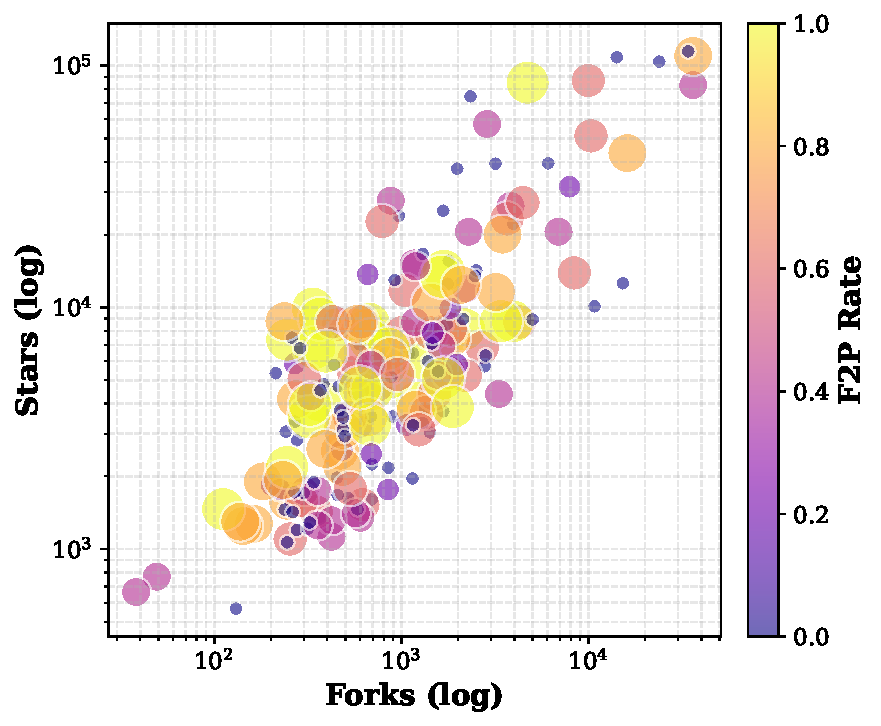
\includegraphics[width=\linewidth]{pic/repo_analysis_kimi_bubble.pdf}
%         \caption{Kimi-K2 Distribution}
%         \label{fig:analysis_star_kimi}
%     \end{subfigure}
%     \hfill
%     % 第三张子图：fork stars gemini-3-flash
%     \begin{subfigure}[b]{0.32\linewidth}
%         \centering
%         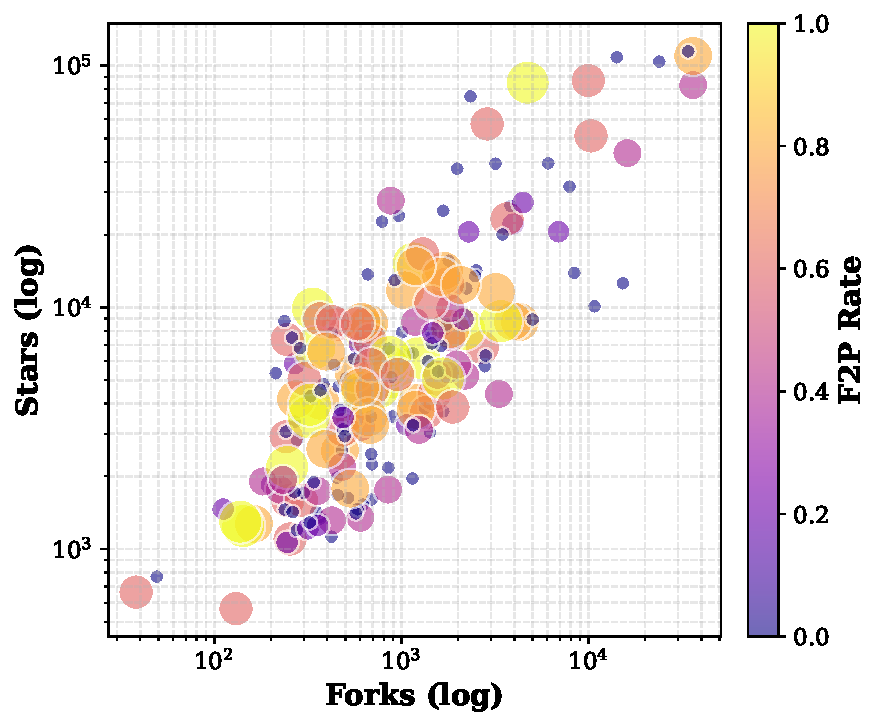
\includegraphics[width=\linewidth]{pic/repo_analysis_gemini_bubble.pdf}
%         \caption{Gemini-3-Flash Distribution}
%         \label{fig:analysis_star_gemini}
%     \end{subfigure}
    
%     \caption{F2P performance analysis relative to repository metrics. (a) Impact of repository size on average F2P rate, showing a clear declining trend as scale increases. (b-c) Distribution of F2P rates for Kimi-k2 and Gemini-3-Flash across varying Star and Fork counts. Results indicate that repository scale is a more significant bottleneck than community popularity.}
%     \label{fig:performance_analysis}
%     \vspace*{-0.5cm} 
    
% \end{figure*}




\paragraph{Component Effectiveness.}
We analyze the contribution of each component in Table~\ref{tab:ablation_main}. MEnvAgent achieves optimal performance across all metrics, validating the synergy between retrieval and patching. Specifically, removing the EnvPatchAgent (\textit{w/o EnvPatchAgent}) causes the Reuse Success Rate to drop significantly from 39.0\% to 25.0\%, forcing frequent fallbacks to scratch builds that degrade both the overall Pass Rate (by 7.0\%) and efficiency (by 20\%). This confirms that the EnvPatchAgent is essential for bridging version discrepancies in retrieved environments. Furthermore, compared to the baseline without reuse (\textit{w/o Reuse}), our full framework reduces the average computational time by 46.0\%, demonstrating that the reuse mechanism is the primary driver of efficiency gains while the patching mechanism ensures the validity of the accelerated process.

\begin{table}[h]
    \centering
    \caption{Ablation results on component effectiveness (conducted with 10 instances per repository). \textbf{RSR} denotes the Reuse Success Rate.}
    \label{tab:ablation_main}
    \resizebox{0.95\linewidth}{!}{%
    \begin{tabular}{@{}lccc@{}}
    \toprule
    \textbf{Method} & \textbf{RSR (\%)} & \textbf{PASS (\%)} & \textbf{TIME (s)}  \\ \midrule
    \textbf{MEnvAgent} & \textbf{39.0} &  \textbf{59.0} & \textbf{2314}  \\
    w/o EnvPatchAgent & 25.0& 52.0 & 2777  \\
    w/o Reuse & 0.0 & 40.5 & 4283  \\
    \bottomrule
    \end{tabular}%
    }
\end{table}


% \begin{figure*}[t]
%     \centering
%     \includegraphics[width=\linewidth]{pic/ablation_impact_of_data_scale.pdf}
%     \caption{\textbf{Impact of data scale on performance metrics.} We compare the baseline (w/o Reuse), direct reuse (w/o EnvPatch), and our full method (MEnvAgent) as the number of instances per repository increases.}
%     \label{fig:ablation_trend}
% \end{figure*}

\paragraph{Impact of Data Scale.}
We further investigate how the volume of historical data influences performance by scaling the number of instances per repository from 1 to 10, as shown in Figure~\ref{fig:ablation_trend}. In sparse data settings (1 instance), the Reuse Success Rate is negligible, resulting in performance similar to the scratch baseline. However, as the data scale expands to 10 instances, the Reuse Success Rate rises steadily to 39\%, driving concurrent improvements in Pass Rate and corresponding reductions in Time Cost. 
This trend highlights the scalability of our approach, suggesting that in real-world scenarios characterized by large-scale data accumulation, the framework is poised to deliver even greater efficiency gains.

\subsection{In-depth Result Analysis}

\paragraph{Performance vs. Repository Scale.}
Figure~\ref{fig:f2p_repo_size} analyzes the correlation between model performance and repository characteristics. We observe a significant negative correlation between Fail-to-Pass (F2P) rates and repository size. This trend is attributable to the intricate dependency graphs and substantial build overheads inherent in large-scale projects, which exacerbate the complexity of automated environment configuration. 
Interestingly, performance exhibits no discernible correlation with community popularity metrics such as Stars or Forks. Notably, bottlenecks persist even in high-star repositories, suggesting that these projects often entail greater architectural complexity and stricter testing standards, thereby posing more rigorous challenges to the reasoning and generalization capabilities of current LLMs.
\begin{figure}[t]
  \centering
  \includegraphics[width=0.7\columnwidth]{pic/repo_size_final.pdf}
  \caption{F2P performance analysis relative to repository size}
  \label{fig:f2p_repo_size}
  \vspace*{-0.25cm}  
\end{figure}



\paragraph{Error Distribution and Behavioral Patterns.}
Figure~\ref{fig:error_dist} categorizes the outcomes of Kimi-k2 and Gemini-3-flash across 10 programming languages into four states: F2P (Fail-to-Pass), P2P (Pass-to-Pass), Test Execution Failure, and Environment Setup Failure. 
Our analysis reveals a significant cross-language performance disparity. Both models achieve high validity in Go and Python (F2P $>50\%$), benefiting from standardized package management ecosystems. In contrast, they struggle with C++ and Java, where environment setup failure rates spike to 52\% due to complex, implicit dependency chains. In terms of model robustness, Gemini-3-Flash consistently maintains lower environment setup failure rates than Kimi-K2. This gap is most pronounced in Java, where Gemini's failure rate (25\%) is nearly half that of Kimi's (47\%), indicating superior generalization in generating complex installation scripts. 
Furthermore, we identify a prevalent bottleneck in C language projects, characterized by a high test execution failure rate (approx. 49\%--57\%). In these cases, mismatches between generated test scripts and project structures lead to validation failures despite successful builds. This high incidence of execution errors underscores the critical necessity of the \textbf{Verification Agent} within the MEnvAgent framework for precise error attribution and iterative refinement.
\begin{figure}[t]
  \centering
  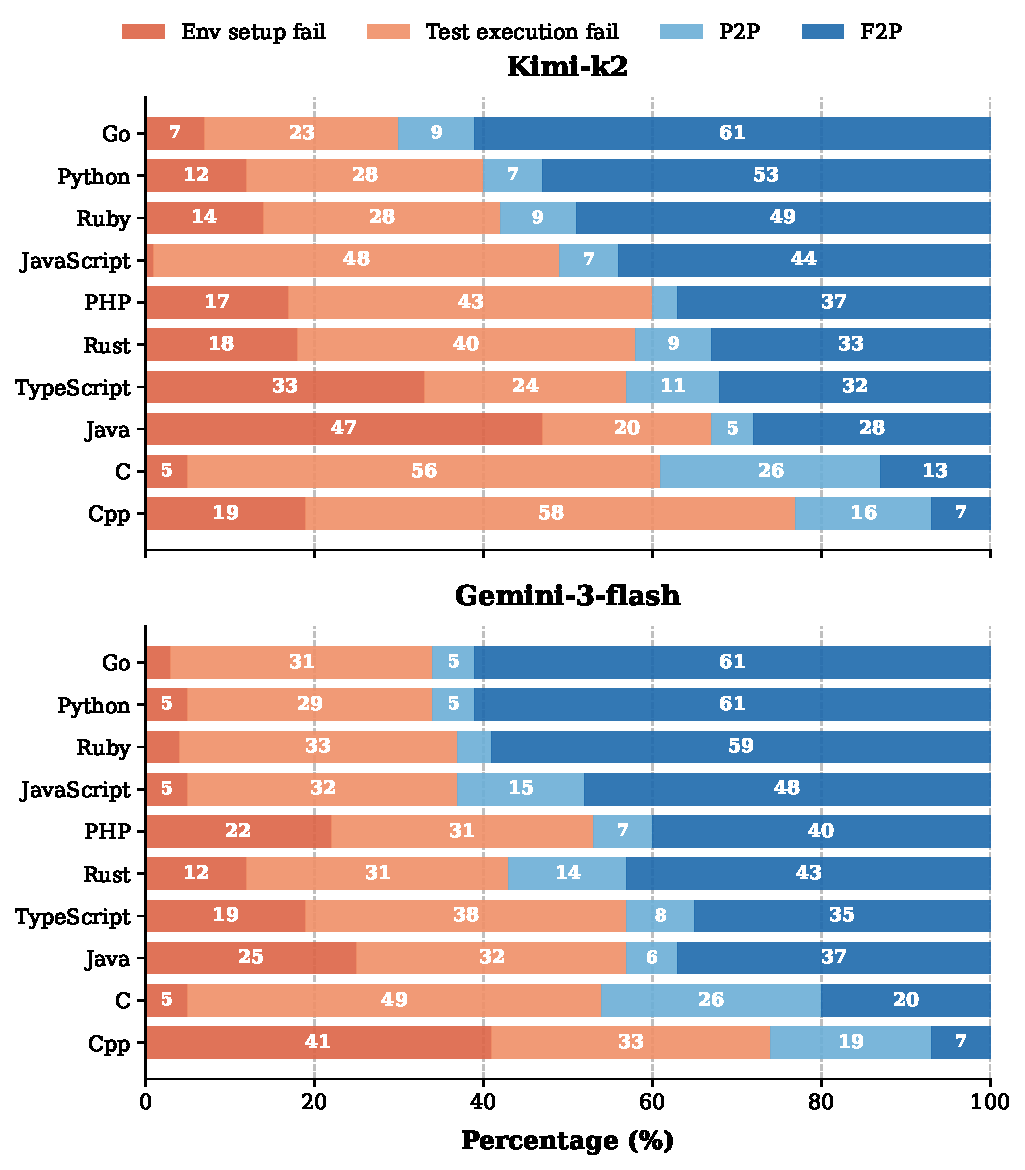
\includegraphics[width=\columnwidth]{pic/error_distribution_combined.pdf}
  \caption{Error distribution across 10 programming languages. (a-b) The percentage breakdown of task outcomes: F2P, P2P, Test execution failure, and Environment setup failure. }
  \label{fig:error_dist}
  \vspace*{-0.25cm}  
\end{figure}
% ---------------- Figures ----------------

% \begin{figure*}[t]
%     \centering
%     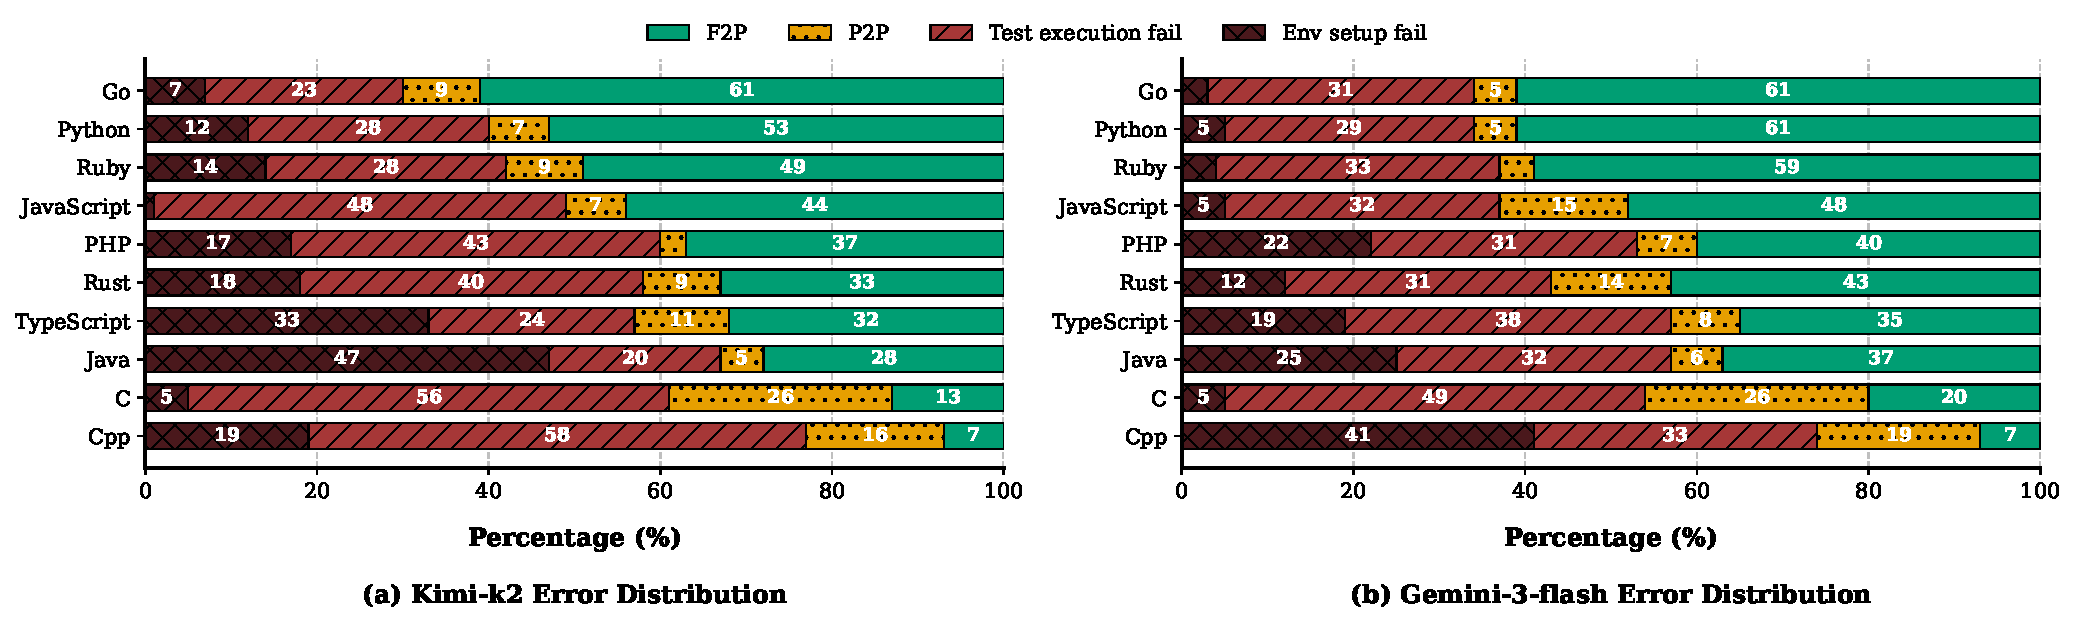
\includegraphics[width=1.0\linewidth]{pic/ordered_comparison.pdf}
%     \caption{\textbf{Error distribution across 10 programming languages.} (a-b) The percentage breakdown of task outcomes: F2P, P2P, Test execution failure, and Environment setup failure. Results highlight that low-level languages like C++ present significantly higher setup challenges compared to modern high-level languages like Go.}
%     \label{fig:error_dist}
% \end{figure*}

% \begin{figure*}[t]
%     \centering
%     % 第一张子图：scale
%     \begin{subfigure}[b]{0.49\linewidth}
%         \centering
%         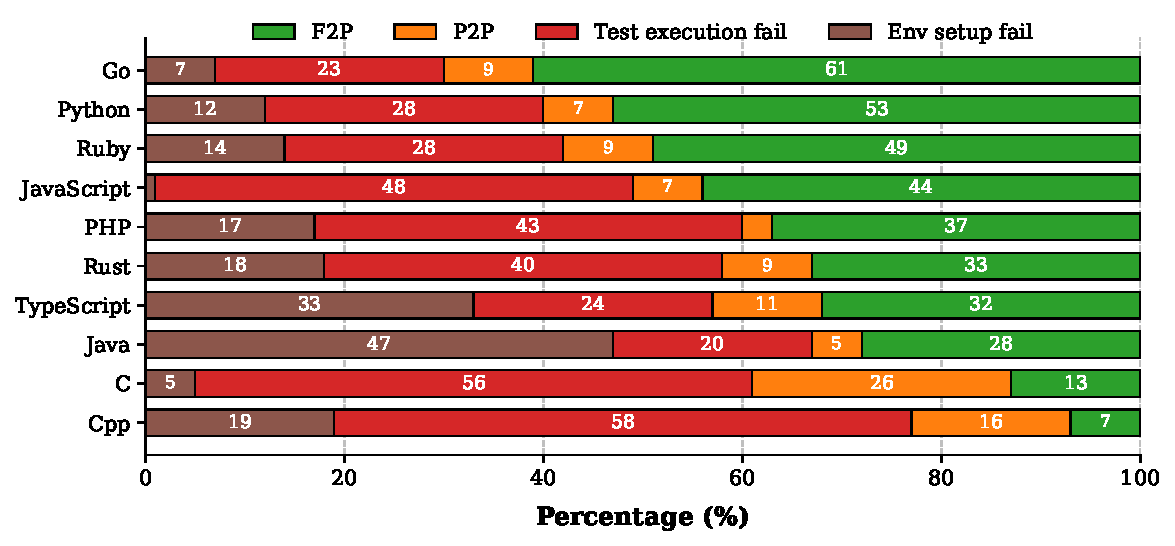
\includegraphics[width=\linewidth]{pic/error_distribution_kimi.pdf}
%         \caption{Kimi-K2 Error Distribution}
%         \label{fig:error_kimi}
%     \end{subfigure}
%     \hfill
%     % 第二张子图：fork stars kimi-k2
%     \begin{subfigure}[b]{0.49\linewidth}
%         \centering
%         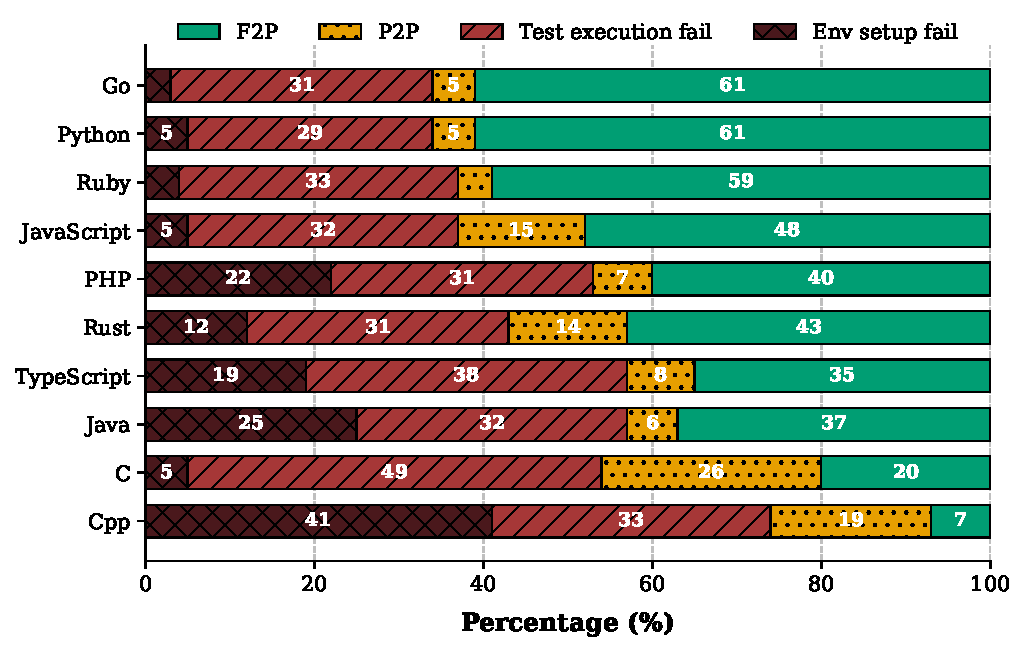
\includegraphics[width=\linewidth]{pic/error_distribution_gemini.pdf}
%         \caption{Gemini-3-Flash Error Distribution}
%         \label{fig:error_gemini}
%     \end{subfigure}
%     \caption{\textbf{Error distribution across 10 programming languages.} (a-b) The percentage breakdown of task outcomes: F2P, P2P, Test execution failure, and Environment setup failure. Results highlight that low-level languages like C++ present significantly higher setup challenges compared to modern high-level languages like Go.}
%     \label{fig:error_dist}
%     \vspace*{-0.5cm} 
% \end{figure*}
\section{Related Work}
% \paragraph{Environment Configuration Agent.}
\paragraph{Agent Method.}
% 早期一些启发式工作
Early attempts at automated environment setup primarily relied on static heuristics to infer dependencies from source code, offering determinism but struggling with intricate system configurations and version incompatibilities \citep{gruber_flapy_2023,zhang_codeagent_2024,badertdinov2024scaling}. 
% 随着大语言模型的发展，出现一系列基于大语言模型的自动化方法，能引用的，都引用；
With the rapid evolution of Large Language Models (LLMs), a series of LLM-based automated approaches have emerged to address these limitations\citep{bouzenia_you_2025,milliken_beyond_2025,vergopoulos_automated_2025,badertdinov_swe-rebench_2025}.
Among the most state-of-the-art and relevant works, Repo2Run\cite{hu_repo2run_2025} employs a dual-agent framework tailored with Python-specific tools, focusing exclusively on environment installation via fixed test commands that do not execute verification tests. Similarly, SWE-bench-live\cite{zhang_swe-bench_2025} extends the task scope to encompass both environment setup and test configuration, utilizing a single-agent method operating via interactive bash sessions. In contrast, SWE-factory\cite{guo_swe-factory_2025} further broadens applicability by supporting four programming languages, introducing a collaborative multi-agent architecture for automated environment construction.

% \paragraph{Environment Configuration Benchmarks.}
\paragraph{Benchmarks.}
Initial efforts evaluated the capability of environment construction implicitly within comprehensive tasks\cite{bogin_super_2024,siegel_core-bench_2024,tang_ml-bench_2024}, offering little insight into the isolated challenges LLMs face during the construction phase.
To explicitly assess this capability, dedicated benchmarks emerged: INSTALLAMATICBench\cite{milliken_beyond_2025} and EXECUTIONAGENTBench\cite{bouzenia_you_2025} established rigorous execution-based standards but remained small-scale. 
Conversely, EnvBench\cite{eliseeva_envbench_2025} and Repo2Run-bench\cite{hu_repo2run_2025} scaled up data but relied on approximate evaluation metrics like static compilation checks or test collection which often fail to detect runtime incompatibilities essential for robust agent feedback.
To further enhance diagnostic depth, EnConda-Bench\cite{kuang_process-level_2025} introduces process-level diagnostics, yet it remains restricted to Python and rigid configuration patterns. 
Notably, SweSetupBench-lite\cite{guo_swe-factory_2025} aligns evaluation with realistic software evolution by supporting historical repository states and adopting metrics like Fail-to-Pass (F2P) rates and efficiency costs. While these features suit scalable evaluation scenarios and capture dependency drift, the representativeness of benchmark is hindered by a narrow scope of only 12 repositories.
\section{Conclusion}

In this paper, we introduced MEnvAgent, a scalable and polyglot framework that automates the complex task of environment construction through a multi-agent Plan-Execute-Validation architecture. A critical advancement of our approach is the novel Environment Reuse Mechanism, which employs an EnvPatchAgent to incrementally update existing environments, thereby resolving the dilemma between build quality and efficiency while supporting diverse technology stacks. We rigorously evaluated our framework on MEnvBench, a new benchmark comprising 1,000 tasks across 10 programming languages, where MEnvAgent demonstrated superior performance, achieving significantly higher validity rates and lower time costs compared to state-of-the-art baselines. By openly releasing the framework and the MEnvData-SWE dataset, we provide the community with essential resources to advance dynamic verification and facilitate future research in Reinforcement Learning with Verifiable Rewards (RLVR) for software engineering.


\newpage
\bibliography{example_paper}
\bibliographystyle{icml2026}
\newpage
\appendix
\onecolumn
%%%%%%%%%%%%%%%%%%%%%%%%%%%%%%%%%%%%%%%%%%%%%%%%%%%%%%%%%%%%%%%%%%%%%%%%%%%%%%%
%%%%%%%%%%%%%%%%%%%%%%%%%%%%%%%%%%%%%%%%%%%%%%%%%%%%%%%%%%%%%%%%%%%%%%%%%%%%%%%
% APPENDIX
%%%%%%%%%%%%%%%%%%%%%%%%%%%%%%%%%%%%%%%%%%%%%%%%%%%%%%%%%%%%%%%%%%%%%%%%%%%%%%%
%%%%%%%%%%%%%%%%%%%%%%%%%%%%%%%%%%%%%%%%%%%%%%%%%%%%%%%%%%%%%%%%%%%%%%%%%%%%%%%
\section*{Appendix}
The appendix of this paper is organized as follows. 

\section{Details of the Automated SWE Tasks Production Pipeline}\label{append:data_production}

In this section, we provide a comprehensive description of the automated pipeline established to construct the high-quality, environment-aware SWE dataset. The pipeline transforms raw repositories into verified software engineering tasks through four sequential stages: (1) Data Collection and Filtering, (2) Automated Quality Evaluation, (3) Environment Construction via MEnvAgent, and (4) Execution-based Verification.

\subsection{Data Collection and Filtering}
The initial phase involves harvesting potential tasks from GitHub. We target repositories and Issue-Pull Request (PR) pairs that meet strict quality criteria to ensure the dataset's relevance and complexity.

\paragraph{Repository Selection.}
We crawl GitHub to identify high-quality repositories. To ensure the project's maturity and community engagement, a repository is selected only if it satisfies the criteria listed in Table~\ref{tab:filter_rules} (Top). Specifically, we enforce a primary language ratio of $\ge$ 60\% to ensure the repository is representative of a specific language ecosystem.

\paragraph{Instance Extraction and Filtering.}
From the selected repositories, we extract Issue-PR pairs (referred to as \textit{instances}). An instance is defined as a closed Issue linked to a merged PR. To ensure the task is solvable and computationally feasible for LLM agents, we apply a set of heuristic rules shown in Table~\ref{tab:filter_rules} (Bottom). Notably, we strictly require the presence of both test patches and fix patches, and limit the patch size ($\le$ 1,000 lines) to focus on functional bug fixes rather than large-scale refactoring.

% [优化] 小表格在单栏模式下不要撑满全宽，0.65左右比较美观
\begin{table}[h]
\centering
\caption{Filtering criteria for Repositories and Instances.}\label{tab:filter_rules}
\resizebox{0.65\linewidth}{!}{%
\begin{tabular}{llc}
\toprule
\textbf{Scope} & \textbf{Metric / Criteria} & \textbf{Threshold} \\
\midrule
\multirow{4}{*}{\textbf{Repository}} 
 & Popularity (Stars) & $\ge$ 1,000 \\
 & Primary Language Ratio & $\ge$ 60\% \\
 & Community Activity (Forks, Issues, PRs) & $\ge$ 200 each \\
\midrule
\multirow{6}{*}{\textbf{Instance}} 
 & Issue Status & Closed \\
 & Problem Description & Non-empty \\
 & Test Patch \& Fix Patch & Non-empty \\
 & Code Modification & Required \\
 & Patch Size (Lines of Code) & $\le$ 1,000 \\
 & Scope (Number of Files) & $\le$ 10 \\
\bottomrule
\end{tabular}%
}
\end{table}

\subsection{Automated Quality Evaluation}
Heuristic filtering alone cannot guarantee the semantic quality of the issue descriptions. To filter out tasks with vague descriptions or irrelevant discussions, we employ an LLM-based evaluator (e.g., DeepSeek-V3.2) to assess the quality of each issue. The model acts as a judge, rating the clarity and completeness of the problem description. The prompt template used for this evaluation is presented in Figure~\ref{fig:quality_prompt}.

% [优化] figure* 改为 figure
\begin{figure}[t]
\centering
\begin{tcolorbox}[
    colback=white,
    colframe=gray!60,
    title=\textbf{Prompt for Issue Quality Evaluation},
    coltitle=white,
    boxrule=0.8pt,
    arc=2pt,
    width=\linewidth
]
\small

\textbf{Role Definition} \\
You are an experienced software engineer. You need to evaluate the quality of an Issue to determine if it contains sufficient information for an engineer to unambiguously provide a solution.

\vspace{0.5em}
\textbf{Issue Scoring Standards} \\
The full score is 10 points (Excellent quality: clear description, explicit requirements for the solution), and 0 points indicates very poor quality (impossible to understand the problem). \\
\textit{Note: If a solution cannot be implemented based on the Issue, the score should not exceed 5.}

\vspace{0.5em}
\textbf{Deduction Rules} \\
Check for deduction items item by item. If the issue has problems or violates the standards, point it out and deduct points in the subsequent evaluation.

\textbf{1. Major Deductions (Violating any item results in a 5-point deduction):}
\begin{itemize}[leftmargin=15pt, topsep=2pt, itemsep=0pt, parsep=0pt]
    \item \textit{Key Information Missing:}
    (1) Lack of expected results: No description of correct behavior/output; for data processing, missing input examples and expected/error outputs.
    (2) Lack of reproduction steps: No operation flow or runnable code to reproduce the issue.
    (3) Missing version info: Unspecified libraries, frameworks, OS, or environment details.
    (4) Incomplete error logs: Snippets provided without context or stack traces.
    \item \textit{Non-Issue Type Submission:}
    (1) Misuse of PR description: Using Pull Request description text directly as an Issue.
    (2) Solved problem: The problem described is already fixed or closed.
    (3) Non-problem inquiry: Content involves release plans, future feature questions, etc., rather than actual defects.
\end{itemize}

\textbf{2. Common Deductions (Deduct points based on severity):}
\begin{itemize}[leftmargin=15pt, topsep=2pt, itemsep=0pt, parsep=0pt]
    \item \textit{Unclear Description:}
    (1) Mixed problems: Single Issue contains multiple unrelated problems or logical contradictions.
    (2) Undefined terminology: Uses unexplained jargon or abbreviations.
    (3) Unquantified requirements: Uses vague descriptions (e.g., "reasonable defaults", "user-friendly", "faster") without measurable acceptance criteria.
    (4) Low-quality test cases: Insufficient, overly broad, or missing test cases (passing the test does not prove the issue is resolved).
    \item \textit{Excessive Reliance on External Resources:}
    (1) Core info relies on external links: Key descriptions/logs/steps are in links that may fail or be inaccessible.
    (2) Reliance on private repos: Reproduction depends on non-public codebases.
\end{itemize}

\vspace{0.5em}
\textbf{Input Content} \\
Issue \\
\textcolor{blue}{\{issue\}}

\vspace{0.5em}
\textbf{Output Format} \\
Please provide your professional analysis and strictly output a number in the following format: \\
reason for evaluation: xxx \\
issue score: 0-10

\end{tcolorbox}
\caption{The prompt template used for the deduction-based Issue quality evaluation.}\label{fig:quality_prompt}
\end{figure}

\subsection{Environment Construction}
This phase constitutes the core of our pipeline, where \textbf{MEnvAgent} is deployed to automatically retrieve codebases, resolve dependencies, and generate Docker images. 

Environment construction is the most computationally intensive and time-consuming component of the pipeline, serving as the primary performance bottleneck. 
On standard local infrastructure, the Docker daemon severely limits concurrent build operations; our preliminary benchmarks indicate that effective concurrency is capped at approximately 10--15 tasks. Given that resolving complex dependencies for legacy repositories can span several hours per instance, achieving large-scale dataset generation on local machines is virtually infeasible.

To overcome this scalability barrier, we re-engineered the underlying infrastructure to support Kubernetes (K8s) orchestration. By decoupling the build agents from the host limits, we achieved (1,000+ parallel builds). This architectural shift enabled the rapid construction of thousands of environment-aware images in a short timeframe. We commit to open-sourcing this high-throughput build infrastructure and the resulting data to accelerate community research in large-scale software engineering.

\subsection{Execution-based Verification}
Once the environments are constructed, we verify their validity to ensure they represent genuine, reproducible bug-fix scenarios.

\paragraph{Fail-to-Pass (F2P).}
We implement a rigorous \textit{Fail-to-Pass} verification protocol using test cases extracted from the original Pull Requests. A task is deemed a valid SWE task only if it satisfies the following two-stage strict check:
\begin{enumerate}
    \item \textbf{Reproduction Phase (Fail):} The test script is executed in the environment with only the \textit{Test Patch} applied (simulating the buggy state). The outcome must be a \textbf{Failure}, confirming that the reported issue is reproducible within the environment.
    \item \textbf{Verification Phase (Pass):} The test script is executed in the environment with both the \textit{Test Patch} and the \textit{Fix Patch} applied (simulating the fixed state). The outcome must be a \textbf{Success}, confirming that the provided patch effectively resolves the issue.
\end{enumerate}

Only instances that survive this rigorous pipeline are included in the final dataset, guaranteeing that every sample is grounded in a reproducible, executable environment.

%%%%%%%%%%%%%%%%%%%%%%%%%%%%%%%%%%%%%%%%%%%%%%%%%%%%%%%%%%%%%%%%%%%%%%%%%%%%%%%
%%%%%%%%%%%%%%%%%%%%%%%%%%%%%%%%%%%%%%%%%%%%%%%%%%%%%%%%%%%%%%%%%%%%%%%%%%%%%%%
\section{Detailed Results on MEnvBench}\label{append:detailed_results}

Table~\ref{tab:longbench_full} provides the comprehensive performance breakdown across all 10 programming languages evaluated in MEnvBench. The table reports Fail-to-Pass Rate (F2P), Pass Rate (PASS), and Time Cost (TIME) for all compared methods using both Kimi-K2 and Gemini-3-Flash backbones.

% [优化] table* 改为 table，保留 \textwidth 宽度，这在单栏下非常清晰
\begin{table}[h]
\centering
\caption{Detailed performance comparison on MEnvBench across 10 languages. \textbf{F2P}, \textbf{Pass}, and \textbf{Time} denote Fail-to-Pass (\%), Pass Rate (\%), and Average Time Cost (s), respectively. ``-'' indicates the method is not applicable to the specific language.}
\label{tab:longbench_full}
\resizebox{\textwidth}{!}{%
\begin{tabular}{lccccccccccccccc}
\toprule
% =====================================================================================
%                                    PART 1: 前 5 种语言
% =====================================================================================
\multirow{2}{*}{\textbf{Method}} & 
\multicolumn{3}{c}{\textbf{Python}} & 
\multicolumn{3}{c}{\textbf{Go}} & 
\multicolumn{3}{c}{\textbf{Java}} & 
\multicolumn{3}{c}{\textbf{JavaScript}} & 
\multicolumn{3}{c}{\textbf{C}} \\
\cmidrule(lr){2-4} \cmidrule(lr){5-7} \cmidrule(lr){8-10} \cmidrule(lr){11-13} \cmidrule(lr){14-16}
 & F2P & PASS & TIME & F2P & PASS & TIME & F2P & PASS & TIME & F2P & PASS & TIME & F2P & PASS & TIME \\
\midrule

% ----------- Kimi-K2 -----------
\rowcolor{gray!15} \multicolumn{16}{c}{\textit{Kimi-K2}} \\
Repo2Run          & 24 & 26 & 3112 & \multicolumn{3}{c}{-} & \multicolumn{3}{c}{-} & \multicolumn{3}{c}{-} & \multicolumn{3}{c}{-} \\
SWE-Bench-Live        & 13 & 15 & 2589 & 3 & 6 & 4382 & 6 & 13 & 6231 & 11 & 16 & 4725 &  \multicolumn{3}{c}{-}  \\
SWE-Factory       & 31 & 37 & 5512 & 50 & 57 & 5742 & 13 & 16 & 6182 & 37 & 40 & 5650 & 13 & 35 & 5777 \\
\rowcolor{blue!5}\textbf{MEnvAgent} & \textbf{53} & \textbf{60} & \textbf{2311} & \textbf{61} & \textbf{70} & \textbf{3171} & \textbf{28} & \textbf{33} & \textbf{4909} & \textbf{44} & \textbf{51} & \textbf{3210} & \textbf{13 }& \textbf{39} & \textbf{3364} \\

% ----------- Gemini-3-Flash -----------
\rowcolor{gray!15} \multicolumn{16}{c}{\textit{Gemini-3-Flash}} \\
Repo2Run       & 27 & 32 & 3769   & \multicolumn{3}{c}{-} & \multicolumn{3}{c}{-} & \multicolumn{3}{c}{-} & \multicolumn{3}{c}{-} \\
SWE-Bench-Live        & 21 & 23 & 2547 & 13 & 15 & 3689 & 8 & 10 & 5146 & 13 & 24 & 2441 &  \multicolumn{3}{c}{-}  \\
SWE-Factory        &  44& 51 &  5529&  53& 61 & 5193 &  18& 24 & 6582 & 39 & 41 &5690  & 18 & 37 & 5482  \\
\rowcolor{blue!5}\textbf{MEnvAgent}  & \textbf{61} & \textbf{66} & \textbf{2530} & \textbf{61} &\textbf{66} & \textbf{3173} & \textbf{37} & \textbf{43} & \textbf{4797} & \textbf{48} & \textbf{63} & \textbf{3715} & \textbf{20} & \textbf{46} & \textbf{4598} \\
\midrule

% =====================================================================================
%                                    PART 2: 后 5 种语言
% =====================================================================================
\multirow{2}{*}{\textbf{Method}} & 
\multicolumn{3}{c}{\textbf{C++}} & 
\multicolumn{3}{c}{\textbf{Rust}} & 
\multicolumn{3}{c}{\textbf{TypeScript}} & 
\multicolumn{3}{c}{\textbf{PHP}} & 
\multicolumn{3}{c}{\textbf{Ruby}} \\
\cmidrule(lr){2-4} \cmidrule(lr){5-7} \cmidrule(lr){8-10} \cmidrule(lr){11-13} \cmidrule(lr){14-16}
 & F2P & PASS & TIME & F2P & PASS & TIME & F2P & PASS & TIME & F2P & PASS & TIME & F2P & PASS & TIME \\
\midrule

% ----------- Kimi-K2 -----------
\rowcolor{gray!15} \multicolumn{16}{c}{\textit{Kimi-K2}} \\
Repo2Run          & \multicolumn{3}{c}{-} & \multicolumn{3}{c}{-} & \multicolumn{3}{c}{-} & \multicolumn{3}{c}{-} & \multicolumn{3}{c}{-} \\
SWE-Bench-Live        &  \multicolumn{3}{c}{-}  & 11 & 15 & 7142 & 5 & 6 & 7867 &  \multicolumn{3}{c}{-}  & \multicolumn{3}{c}{-}  \\
SWE-Factory       &  \textbf{7}&  21& 5832 &  19&  32& 7773 & 23 & 27 &8962  &30  & 34  & 5759 & 39 & 46 & 6368 \\
\rowcolor{blue!5}\textbf{MEnvAgent} & \textbf{7} & \textbf{23} & \textbf{5254} & \textbf{33} & \textbf{42} & \textbf{4662}
 & \textbf{32} & \textbf{43} & \textbf{2330} & \textbf{37} & \textbf{40} & \textbf{2394} & \textbf{49} & \textbf{58} &  \textbf{1782} \\

% ----------- Gemini-3-Flash -----------
\rowcolor{gray!15} \multicolumn{16}{c}{\textit{Gemini-3-Flash}} \\
Repo2Run          & \multicolumn{3}{c}{-} & \multicolumn{3}{c}{-} & \multicolumn{3}{c}{-} & \multicolumn{3}{c}{-} & \multicolumn{3}{c}{-} \\
SWE-Bench-Live    &  \multicolumn{3}{c}{-}  & 21 & 25 & 5484 & 10 & 18 & 5187 &  \multicolumn{3}{c}{-}  & \multicolumn{3}{c}{-}  \\
SWE-Factory        &  6 & 24 & \textbf{5361} & 37 & 42 &7311  & 24 & 28 & 8050 & 39 & 45 &  5969& 55& 62 & 6582  \\
\rowcolor{blue!5}\textbf{MEnvAgent}  & \textbf{7} & \textbf{26} & 5995 & \textbf{43} & \textbf{57} & \textbf{4828} & \textbf{35} & \textbf{43} & \textbf{3632} & \textbf{40} & \textbf{47} & \textbf{2415} & \textbf{59} & \textbf{63} & \textbf{2399}\\
\bottomrule
\end{tabular}%
}
\end{table}

\section{Detailed hyperparameter settings for MEnvAgent and baselines on MEnvBench.}
\label{append:experiment_setup}

All experiments were conducted on the MEnvBench benchmark. Unless otherwise specified, we used a fixed temperature of 0.5 and a global timeout of 3 hours per task to ensure fair comparison. The detailed hyperparameter configurations for MEnvAgent and all baseline methods are summarized in Table~\ref{tab:hyperparameters}.

\begin{table}[h]
    \centering
    \caption{Detailed hyperparameter settings for MEnvAgent and baselines on MEnvBench. }
    \label{tab:hyperparameters}
    % [修改点] 将宽度从 0.7\linewidth 改为 0.55\linewidth，使其更紧凑
    \resizebox{0.4\linewidth}{!}{%
    \begin{tabular}{llc}
        \toprule
        \textbf{Method} & \textbf{Parameter} & \textbf{Value} \\
        \midrule

        % ---------------- Repo2Run ----------------
        \multirow{4}{*}{\textbf{Repo2Run}} 
        & Max Iterations & 50 \\
        & Time Limit & 3 hours \\
        & Temperature & 0.5 \\
        & Concurrency & 15 \\
        \midrule
        % ---------------- SWE-Bench-Live ----------------
        \multirow{5}{*}{\textbf{SWE-Bench-Live}} 
        & Max Install Iterations & 20 \\
        & Max verify Iterations & 20 \\
        & Time Limit & 3 hours \\
        & Temperature & 0.5 \\
        & Concurrency & 15 \\
        \midrule
        % ---------------- SWE-Factory ----------------
        \multirow{4}{*}{\textbf{SWE-Factory}} 
        & Max Iterations & 5 \\
        & Time Limit & 3 hours \\
        & Temperature & 0.5 \\
        & Concurrency & 15 \\
        % ---------------- MEnvAgent ----------------
        \midrule
                \multirow{4}{*}{\textbf{MEnvAgent (Ours)}} 
        & Max Iterations & 5 \\
        & Time Limit & 3 hours \\
        & Temperature & 0.5 \\
        & Concurrency & 15 \\
        \bottomrule
    \end{tabular}%
    }
\end{table}


\section{Training Implementation Details}
\label{append:training_details}

We fine-tune all models using a unified supervised fine-tuning (SFT) framework based on Megatron-LM. To equip the models with long-context capabilities, we scale the training sequence length to \textbf{128k} tokens ($131,072$).

\paragraph{Optimization and Hyperparameters.}
We employ the \textbf{AdamW} optimizer with a global batch size of $8$. The learning rate is scheduled with a constant strategy, where the peak learning rate is set to $1\times 10^{-5}$ and decays to a minimum of $1\times 10^{-9}$, with no warmup steps. We set the gradient clipping norm to $1.0$ and use a weight decay of $0.1$. For MoE-based models, we apply an auxiliary loss with a coefficient of $1\times 10^{-3}$ to ensure load balancing among experts.

\paragraph{Infrastructure and Efficiency.}
To efficiently train large-scale models with such long contexts, we utilize a comprehensive \textbf{3D parallelism} strategy, configuring Tensor Parallelism (TP), Pipeline Parallelism (PP), and Expert Parallelism (EP) all to size $8$, alongside Sequence Parallelism. Furthermore, we leverage \textbf{Flash Attention 2} to accelerate attention computation and enable full \textbf{activation checkpointing} (recompute) to significantly reduce memory fragmentation during training.
\end{document}

% This document was modified from the file originally made available by
% Pat Langley and Andrea Danyluk for ICML-2K. This version was created
% by Iain Murray in 2018, and modified by Alexandre Bouchard in
% 2019 and 2021 and by Csaba Szepesvari, Gang Niu and Sivan Sabato in 2022.
% Modified again in 2023 and 2024 by Sivan Sabato and Jonathan Scarlett.
% Previous contributors include Dan Roy, Lise Getoor and Tobias
% Scheffer, which was slightly modified from the 2010 version by
% Thorsten Joachims & Johannes Fuernkranz, slightly modified from the
% 2009 version by Kiri Wagstaff and Sam Roweis's 2008 version, which is
% slightly modified from Prasad Tadepalli's 2007 version which is a
% lightly changed version of the previous year's version by Andrew
% Moore, which was in turn edited from those of Kristian Kersting and
% Codrina Lauth. Alex Smola contributed to the algorithmic style files.
